\documentclass[oneside]{ZJUthesis}
\usepackage{longtable}
\usepackage{fontspec}
\usepackage{minted}
\usepackage{courier}
\setmonofont{Courier New}
\renewcommand{\theFancyVerbLine}{
  \sffamily\textcolor[rgb]{0.5,0.5,0.5}{\scriptsize\arabic{FancyVerbLine}}}

\hypersetup{colorlinks=false}
\begin{document}
\songti
\title{对自动编码器的稀疏惩罚因子研究与分析}
\author{姜楠}
\supervisor{龙胜春~副教授}
\major{计算机科学与技术+自动化1101}
\institute{计算机科学与技术学院}
\submitdate{2015年~6月}
\makeCoverPage
\ZJUfrontmatter
\begin{abstract}
机器学习算法严重依赖于数据的表示形式,优良的数据特征能有效提高实验中的准确率。自动编码器算法是一种非监督学习算法,能直接从数据中获取数据的优良特征表示形式,并且能尽可能减少数据失真现象。为了使自动编码器能学习到更加有效的``稀疏''的特征,一种简单的方法就是在模型的``代价函数''中添加稀疏惩罚项。然而,在当前的科技文献中,很少有对稀疏惩罚项的优劣的实验研究。在本文中,我们采用L1范数、L2范数、Student-t惩罚因子和KL差分因子作为我们主要的稀疏惩罚因子的研究对象。我们对这些惩罚因子按照实验评价标准:重构误差、特征的稀疏度和测试集上正确率来分析它们的功能优劣。实验数据集包括:MNIST、CIFAR-10、SVHN、OPTDIGITS和NORB五个数据集。实验结果表明这些惩罚因子均能产生稀疏特征,优于不添加任何惩罚因子的自动编码器。同时,我们也希望关于此主题的讨论研究能为今后的研究提供一些有用的思路。


\keywords{自动编码器,稀疏惩罚因子,稀疏编码,非监督学习}
\end{abstract}

\begin{Eabstract}
Machine learning algorithms depend heavily on the data representation, which dominates its success in experiment accuracy. Autoencoder model structure is proposed to learn from data a good representation with the least possible amount of distortion. Furthermore, it has been proven that boosting sparsity when learning representation can significantly improve performance on classification tasks and also make the feature vector easy to interpret. One straightforward approach for autoencoder to obtain sparse representation is to impose sparse penalty on its overall cost function. Nevertheless, few comparative analysis has been conducted to evaluate which sparse penalty term works better. In this paper, we adopt L1 norm, L2 norm, Student-t penalties, which are rarely deployed to penalise the hidden unit outputs, and commonly used penalty KL-divergence in the literature. Then, we present a detailed analysis to evaluate which penalty achieves better result in terms of reconstruction error, sparseness of representation and classification performance on test datasets. Experimental study on MNIST, CIFAR-10, SVHN, OPTDIGITS and NORB datasets reveals that all these penalties achieve sparse representation and outperforms representations learned by pure autoencoder on classification performance and sparseness of feature vectors. Moreover, we hope this topics and the practices would provide insights for future research.



\Ekeywords{autoencoder, sparse penalty, sparse coding, unsupervised feature learning}

\end{Eabstract}
\ZJUcontents
\ZJUListofFigures
\ZJUListofTables

\mainmatter
\chapter{绪论}
\section{选题背景与意义}
\subsection{监督学习}
机器学习(Machine Learning)常用方法主要分为有监督学习(Supervised Learning)和无监督学习方法(Unsupervised Learning)。监督学习,主要分为分类算法(Classification)和回归算法(Regression)。分类算法是指从已标记的训练数据中来调整分类器的参数,通过迭代更新参数,使得分类器在训练集达到较低的错误率的过程。在监督学习中,每个样本都是由输入样本(多维数据)和期望的输出值组成。训练过程中,通过分析样本数据,来调整模型参数,并产生一个具有推测功能的分类器,其可以用来对新的测试样例进行预测。监督学习是目前机器学习领域中应用广泛的一种成熟算法,在许多领域有很成功的应用,如语音处理和识别、人脸识别和跟踪、无人驾驶等\cite{DBLP:journals/taslp/DahlYDA12,DBLP:conf/icml/Boulanger-LewandowskiBV12,DBLP:journals/neco/HintonOT06,DBLP:conf/nips/BengioLPL06,DBLP:conf/interspeech/YaoZHSY13,DBLP:conf/interspeech/MikolovKBCK10,DBLP:conf/emnlp/SocherPHNM11} 。尽管如此,监督学习还是有很大的限制。因为现实中存在数据集大多没有标签存在,只有少部分实验数据集已被打标签。采用人工打标签方法费时费力,监督学习算法所能实践的数据集受到限制,同时若是数据集的特征维度过高,数据集样本数量过少,监督学习算法很容易出现过拟合现象。训练算法迭代时间将会呈指数增长,相应的模型参数过多,在训练集中表现十分好,在测试集上的表现非常差。目前监督算法模型主要分类为:人工神经网络(Aritificial Neural Network)、支持向量机(Support Vector Machine)、最邻近算法(k-Nearest Neighbor)等。


\subsection{人工神经网络}
人工神经网络(Artificial Neural Network)起源于上世纪生物神经学科对人脑的学习机制的重大突破发现。通过对神经的模拟和近似,人工神经网络能从结构、功能上模拟生物处理信息的过程。BP(Back Propagation)神经网络模型是一种经典的人工神经网络算法,由输入层(Input Layer)、隐藏层(Hidden Layer)、输出层(Output Layer)构成,如图\ref{fig:nn} 所示。
\begin{figure}[H]
\centering
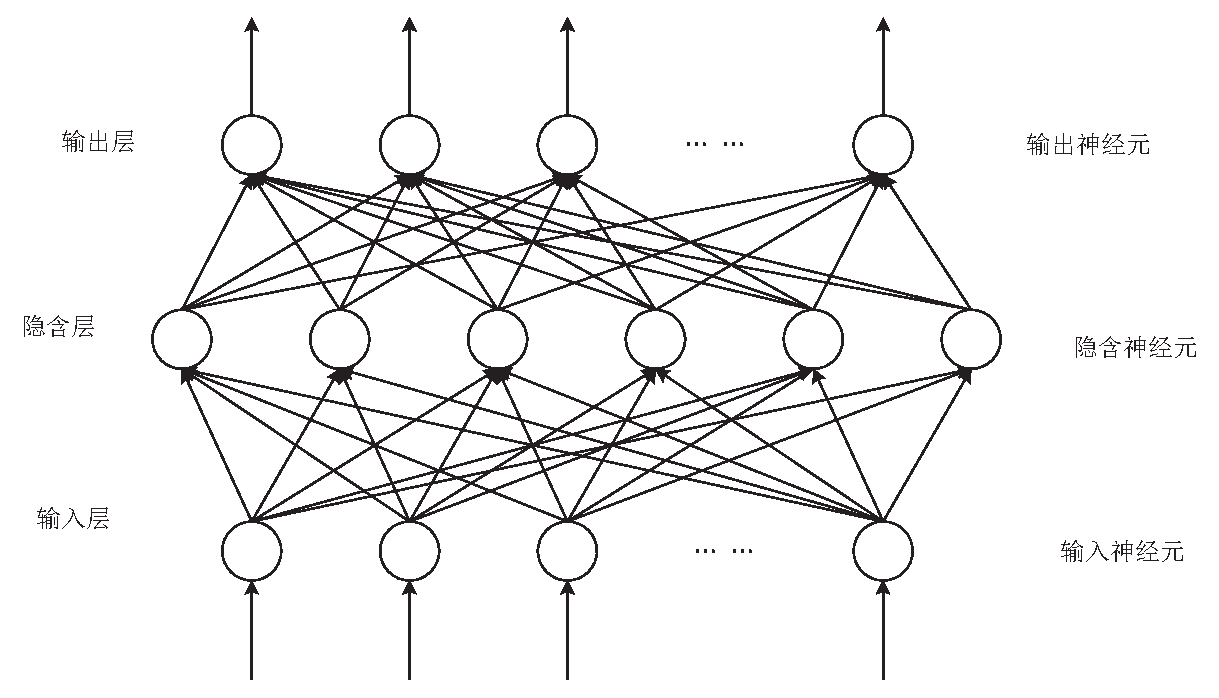
\includegraphics[scale=0.5]{./Pictures/nn.eps}
\caption{典型神经网络结构\label{fig:nn}}
\end{figure}
BP算法由训练过程分为数据流的前向传播和误差信号的反向传播两个过程构成。正向传播时,传递方向为:输入层$\to$ 隐含层 $\to$ 输出层,当前层的神经元能动态影响、更新下一层的神经元节点。若在输出层得不到期望的输出,则转向误差信号的反向传播流程。通过这两个过程的交替进行,动态更新权重向量,使得模型的误差函数随着其梯度方向下降至系统最优解,从而实现了模型的训练过程,即从训练集中提取并记忆了有效信息。BP算法能突破传统多项式公式有限的拟合数据的能力,能学习到更加复杂的非线性函数规律和即使数据中包含一些误差,它也能收敛致最优解,拥有较强的自适应性。

然而,由于BP神经网络的代价函数不是严格意义上的凸函数,一旦算法在迭代优化过程中陷入局部极值,就有可能无法求得系统的最优解。若要拟合高维复杂的函数,采用较复杂的神经网络模型就会导致函数运算量巨大、收敛过慢,若采用较小的神经网络模型,则只能学习到简单的函数方程,可能会忽略了重要的信息特征\cite{1}。


\subsection{非监督学习}
在实际应用中,大多数情况下,获取样本的标签费时费力,只能从原始的无标签数据集入手,需要直接建模原始数据,设计分类器,这个过程称为无监督学习方法(Unsupervised Learning)。有别于监督式学习算法,无监督式学习算法在训练过程中,并不知道其分类结果是否正确,亦即无法告诉它何种学习是正确的。其特点是仅需要提供输入样例,它会自动从样例中找出其潜在类别规则。当学习完成后,可以将其用在全新的样例上。


无监督学习方法可以分为两类,一类为基于概率密度函数估计的方法,它试图找出数据集在特征空间的分布参数,再用特征空间分布进行分类处理。例如稀疏编码算法,它将原始数据压缩表示为字典(Dictionary)的一个线性组合:$x=D*x'$,我们用 $x$ 表示原始信号, $D$ 为我们得到的字典,通过字典 $D$ , 原始信号 $x$ 能被完整地表示为 $x'$ 的线性组合。为了解决字典 $D$ 的退化(Degeneracy)问题,Hinton等人提出了稀疏自编码(Sparse Auto-encoder)学习算法。另一类称为基于样本间的相似性度量的聚类方法,它通过聚类方法将样本划分成不同类别,例如:Kmeans聚类算法。 

\subsection{稀疏自动编码器算法}
稀疏自动编码器算法能实现提取样本中的稀疏特征,是近年提出的一类有效的无监督学习算法。它把原始数据用隐藏层的特征空间向量表示,再把隐藏层特征解码成重构的输出层。这样,隐藏层中的特征信息就是输入层的一个压缩表示,而且有效减少了冗余信息。并且,压缩表示的特征很适合进一步用作分类器的输入集。该模型可以用来标注无标签的数据集,免去了繁复的人工打标签的操作,同时也能有效降低输入数据的维度,防止出现``维度灾难'',即模型的计算时间和计算复杂度会随着维度的增加呈指数倍增长。

当我们将稀疏性概念引入后,即我们希望 $x'$ 是稀疏的,只有较少的非零项,这样做最突出的优点是能有效提升运算速度。在模型选择过程中,我们有多种稀疏因子可以选取,例如$L_p-norm$因子,KL-divergence因子。


\section{国内外研究现状}
原型自动编码器能学习到数据中的非线性特征结构,它能提取出高位复杂的输入数据中的低维特征,将此特征用于深度学习其它模型的输入,能有效提升系统的精确度\cite{16}。
自动编码器模型包括编码和解码两个主要步骤。在编码阶段,编码器将输入数据 $x$ 映射到隐含层特征$h$。在解码阶段,映射函数 $g(h)$ 将隐含层特征空间映射回重构的输入层$\hat x$ 。原型自动编码器模型在运用到实际条件中,演变产生各种修正的模型,按照其主要类别,大致分为:稀疏自动编码器、降噪自动编码器、鲁棒自动编码器和卷积自动编码器\cite{曲建岭2014深度自动编码器的研究与展}。

\subsection{稀疏自动编码器}
对于JPEG图像的压缩算法,原始信号经过离散余弦变换只有,只有极少数原数是非0的,有效降低图片的大小,这就是信号的稀疏性表示。采用压缩形式表示输入信号能更方便地对信号进行加工处理,如信号和图像的采集处理、编码和信息论等。通过对原型自动编码器的隐藏层添加约束条件,并增加隐藏层节点个数,能在隐藏层中获得原始数据的结构性特征。假设自定编码器的输入为$x$,约束项为$\rho$,隐藏层神经元节点的平均激活度记作$\rho_j$。一般地,期望隐藏层的绝大多数神经元的取值在0 附近,少数神经元节点取值接近1,即只有少数神经节点处于激活状态。稀疏自动编码器能提取高位数据中的稀疏性特征,增加数据的线性可分性。然而原始数据分布规律不同,故需要较大的数据集来训练稀疏自动编码器以便完成的获取稀疏特征变量。另外也需要预先调节KL散度的惩罚值,并要求隐藏层的平均激活程度相同,致使实验的效果较差,容易出现欠拟合问题。

\subsection{降噪自动编码器}
降噪自动编码器(Denoising Auto-encoder)是在自动编码器的输入层中加入高斯分布的随机噪声,进而自动编码器在训练过程中,尝试学习去除这种噪声,解码过程中,模型根据噪声统计特性,从未受到干扰的数据中,估计出原始数据的分布规律,从而消除添加的高斯噪声。最终,自动编码器学习到的特征具有更强的鲁棒性,拥有更强的泛化能力\cite{28}。
\begin{figure}[H]
\centering
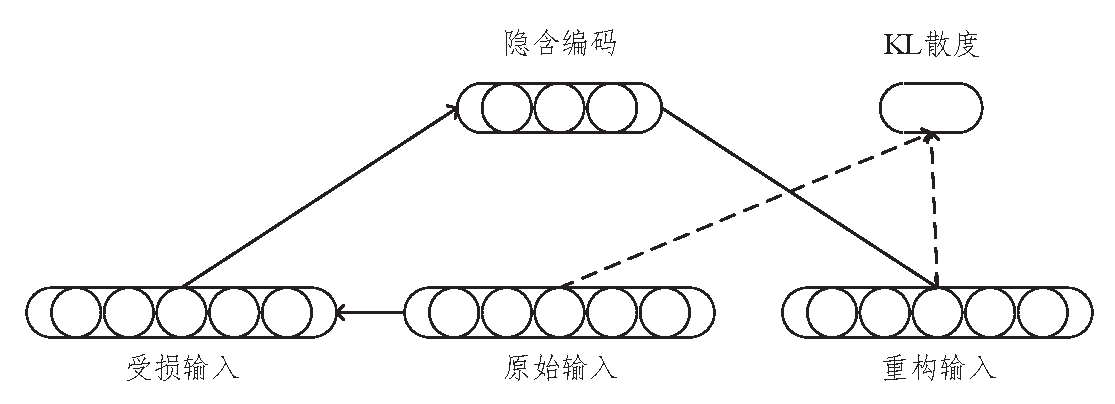
\includegraphics[scale=0.6]{./Pictures/deAE.eps}
\caption{降噪自动编码器模型\label{fig:tanh}}
\end{figure}

\subsection{收缩自动编码器}
\begin{defn}[Frobenius范数]
	对实矩阵 $A=[a_{ij}] \in R^{m*n}$,称非负实数:
	\begin{equation}
	\|A\|_F=\sqrt{\sum\limits_{i=1}^{m}\sum\limits_{j=1}^{n}{a_{ij}^2}}
	\end{equation}
	为A的Frobenius范数,简称F范数。
\end{defn}
当添加Frobenius范数作为惩罚因子后,收缩自动编码器能有效处理输入数据中的小扰动,而且隐藏层重构特征不受惩罚因子约束,有效提高了数据表示的鲁棒特性。可以利用BP算法求解系统的最优解,获得系统的最佳配置参数\cite{32}。

\subsection{卷积自动编码器}
在计算机图像处理领域,卷积自动编码器能有效解决图像中存在的池化和白化问题。上述讨论的模型在应用到图形图像领域后,需要配置大量冗余的参数,计算效率也大大降低。然而卷积自动编码器能获取局部特征,完整保留边缘特征,其算法模型如图\ref{fig:conv}所示。
\begin{figure}[H]
\centering
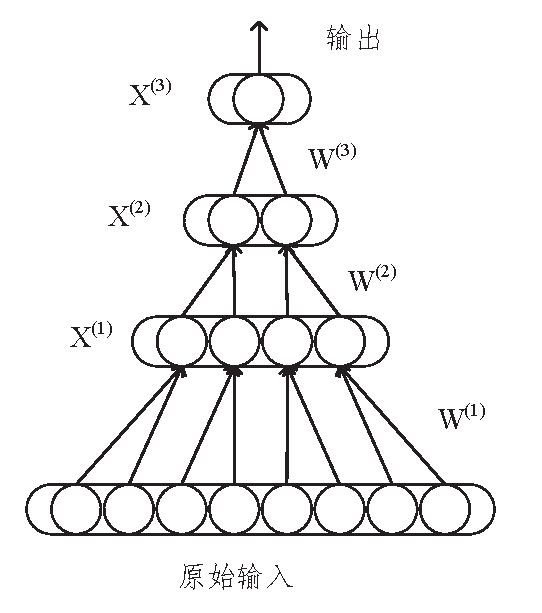
\includegraphics[scale=0.6]{./Pictures/conAE.eps}
\caption{卷积自动编码器模型\label{fig:conv}}
\end{figure}


\section{需要解决的问题及研究内容}
\subsection{需要解决的问题}
1. 随着算法模型的架构变得巨大和神经元节点数量地增加,模型训练时间呈指数级增长。不仅如此,由于模型训练过程中采用梯度反向传播算法来更新权重矩阵,随着深度的增加,误差的二阶导数、三阶导数会越来越小,即所谓的梯度弥散现象,误差反向传播的影响随着深度增加越来越小,从而导致权重矩阵的迭代更新速度变慢,拖慢系统训练时间,使得自动编码器无法拟合一些高维复杂函数\cite{35}。 

自动编码器的训练时间过长,系统参数调优需要很多设计技巧,且人工神经网络中参数的物理意义一直以来难以被合理解释,自动编码器训练获得的特征也是如此,研究人员尚无法认识学习到的特征的物理意义何在。自动编码器算法较为单一,尽管我们可以通过重复使用该模型,不断堆叠,提取相对更深层次的特征,但是理论上的证明尚未完善,无法确证学习获得的特征有助于后续分类器的设计。另一方面,通过简单堆叠获得的深度模型,需要模型整体调优(Fine Tuning)才能达到有效的精确率提升。然而调优过程运算过程更加漫长,无法满足实际开发需要。目前使用的建模手段,即使用自动编码器作为预训练手段,通过堆叠自动编码器提取深层次的特征和深层模型整体调优手段,相比于传统机器学习算法相对单一,无法满足训练复杂网络的需求\cite{40}。

2. 现有的预训练算法对类标签数据集有较强的依赖性,远没有达到``无监督学习''\cite{41}。不仅如此,现有算法对硬件需求极高,模型训练过程中,原始数据矩阵和参数矩阵不断迭代,占用极大内存,同时繁复的矩阵运算考验着系统的并行能力,随着处理数据规模的增大,现有软硬件环境无法满足其需求。使用Navida的图形处理器(GPU),由于其专门提供了 CUDA并行编程环境,用作矩阵并行运算的硬件环境将是大势所趋,若能开发针对特定算法模型的硬件框架,利用高并发的硬件指令实现软件算法将会极大提升算法训练时间,那将革新现有的算法效率\cite{43}。

3. 另一方面,生物神经学科发展远远落后于深度学习发展速度,现有理论的突破需要神经科学的进一步研究成果\cite{36,37}。现有模型仅源于十几年前的生物学人体神经的发现,若能在生物科学上对人脑运作模型有所突破发现,那能帮助我们建立更加可靠的模型和理论。

\subsection{研究内容}
1. 基于稀疏理论的自动编码器是目前应用最为广泛的自动编码器,它能在低维的特征空间内重建高维数据变量,并获得稀疏表示的特征。获得的特征能用于后续的分类器,能有效增强数据的线性可分性,提高了分类器的准确率。本课题的研究目标定位于利用MATLAB技术来实现自学习算法(稀疏自动编码器+Softmax回归模型),着重于讨论并研究稀疏自动编码器中的稀疏惩罚因子(Sparsity Penalty)对该自学习算法的性能表现,我们主要按照三个指标来评价其性能差异:提取特征的稀疏度,测试集上的重构误差,测试集上的精确度。通过研讨其在不同数据集上的性能表现,期望分析出稀疏惩罚因子的实用价值及效用。

2. 为了便于实验操作,故搭建web实验平台,以网络服务形式开放给用户使用。其计算模型是稀疏自动编码器模型,用户可以在实验平台上提交实验的数据集,和选择实验的数据预处理手段,当用户自定义完上述选项后就可以以任务形式提交到实验平台上,网站后台接收到用户的计算请求后,调用硬件资源开始计算。用户可以实时查看计算任务的进展,当任务完成后,平台将实验的数据及实验图表展示给用户。用户可以在线查看实验结果,以便进行后续数据分析。


\chapter{开发环境及框架}
\section{系统开发环境}
现在有许多主流的操作系统,我们应当根据不同的使用需求,合理选择操作系统。例如为众人所熟知的 Win7 操作系统适用于家庭休闲使用,由于其病毒版本较多、对主流开源软件支持较差等原因,不适合选做系统开发环境。一般,我们系统开发、网站建设通常采用较为稳定、高效的 Linux 系统。Linux 开源系统中,又以 CentOS 作为主流的服务器的操作系统。本实验的环境配置为:CentOS 6 操作系统,Intel Xeon 24核 CPU,64GB内存。

CentOS\footnote{CentOS: www.centos.org}是企业级社区操作系统,它是Linux的重要的一个发型系列产品。一直以来,由红帽公司负责维护,开发其更新和修复主要的功能缺陷。 本着开源精神,红帽公司毅然将其开发的著名操作系统RHEL中的稳定的软件代码公开,并建立开发者社区来维护和更新其CentOS的系统架构。考虑到RHEL和CentOS拥有同样的源代码,因此有些企业针对部分服务器安装CentOS操作系统以替代昂贵的商业版的RHEL,CentOS的稳定的网络框架秉承RHEL操作系统的特点能满足苛刻的实践应用。RHEL和CentOS操作系统的主要不同点在,于CentOS并不包含RHEL开发的闭源代码库。CentOS对部分源代码进行修改,以便维护商家版权,减少不必要的纷争。

在此操作系统之上,安装 MATLAB 软件所依赖的Oracle JDK 8。同时本实验所采用的 Django 1.8 开发框架依赖于Python 2.7 和 MySql 6 。均需要预先安装。
\begin{minted}[mathescape,
               numbersep=5pt,
               gobble=2,
               frame=lines,
               framesep=2mm]{Shell}
    sudo apt-get install build-essential  
    sudo yum install python-devel         
    sudo yum install mysql-server         
    sudo pip install django               
\end{minted}
按照代码顺序,我们需要配置安装操作系统的开发环境依赖库,接着我们需要安装python用于语言开发的配置包,然后是安装mysql客户端。最后当我们需要配置网站开发环境,即通过python 的包管理机制 pip 安装 Django。

\section{编程语言和编程环境}
本实验采用 MATLAB Script \footnote{MATLAB: cn.mathworks.com}作为算法模型的实现语言(需要Java JDK支持),采用 Python 2.7 作为实验平台的开发语言,采用主流的Web框架django。主要基于以下考虑:MATLAB中配备丰富的数学函数库,并且MATLAB底层的矩阵运算实现机制均进行了并行优化处理\cite{刘卫国2002按对象分层决策矩阵的逼近理想解法的}。相对于Python的numpy开发库,MATLAB有更高效运算效率,采用Python 脚本语言后台调用 MATLAB 接口函数比采用纯粹的 Python 开发框架能有效增强平台的响应时间。另一方面,尽管 MATLAB 配备了 GUI 开发框架,开发人员能直接拖拽组建搭建实验的界面,针对运算时间较短的程序采用MATLAB GUI是一个很好的选择。然而,本算法的迭代求解最优参数环节耗时巨大,会导致界面长时间无法响应用户的交互需求,同时若采用异步线程维护GUI线程和后台运算线程,会造成不必要的CPU和内存的开销,故采用第三方语言实现平台界面的搭建,Django正是这样的敏捷开发的框架,能在较短的开发周期内实现用户的功能需求。

另外,本实验环境为CentOS操作系统,在配置MATLAB之前,需要配置Oracle Java JDK\footnote{Java Development Kits: www.oracle.com}开发环境。由于Linux/Unix操作系统默认配置open JDK作为替代Sun Java JDK的java开发包,这在通用依赖java的软件中尚未构成问题。然而例如MATLAB,Eclipse,Hadoop等软件必须依赖Sun Java JDK开发包和Sun Java JRE开发环境,故需要配置linux下Sun Java开发环境,以便后续步骤顺利进行。
\begin{minted}[mathescape,
               linenos,
               numbersep=5pt,
               gobble=2,
               frame=lines,
               framesep=2mm]{Shell}
   rpm -ivh jdk-8u25-linux-x64.rpm         
   export JAVAHOME=/usr/java/jdk1.8.025/  
   export PATH=$PATH:$JAVAHOME
\end{minted}
首先我们需要从 Oracle官网下载 Java安装包,需要注意的是我们需要下载支持 Linux 的rpm安装包。接着是使用rpm 包管理器解压安装包,即完成了安装过程。为了其他软件能自动找到我们安装的jdk 软件,我们还需要配置 系统的 \texttt{PATH} 变量,加入java的路径。


为了在终端中能直接使用MATLAB软件,我们还需要在安装完MATLAB软件后对其进行配置:
\begin{minted}[mathescape,
               numbersep=5pt,
               gobble=2,
               frame=lines,
               framesep=2mm]{Shell}
    vim /etc/profile
    export PATH=/opt/MATLAB/2014a/bin:$PATH
    source /etc/profile
    echo $PATH
    alias MATLAB='MATLAB -nodesktop -nodisplay'
\end{minted}
首先我们需要将 MATLAB 的安装路径加入系统环境变量,其次为了便于在终端操作,而不是使用 MATLAB 自带的界面,我们启用 \texttt{-nodisplay -nodisdesktop}这个选项,以便以后续操作的便捷进行。


尽管开源软件GNU Octave能提供与MATLAB同样的计算服务,而且开源软件Octave无需考虑版权、授权证书等商业软件MATLAB的约束,但在许多特殊的数据处理细节上,两个各异程度较大,只能兼容常见的系统函数, Octave 包含的计算函数库远没有 MATLAB 丰富。另一方面,Maltab 自带的数据可视化工具,能直接采用脚本语言操纵图像的绘制,并对图像进行必要的标注和打印,MATLAB提供的MEX编译器能支持C++,python,Java等支流开发语言的混合编译,部分对性能要求严格的函数转而利用C语言实现,能在硬件环境下更高效的执行,通用性远远高于Octave软件。故放弃Octave软件,转而采用MATLAB软件。

历来Python的IDE纷繁复杂,由于其环境配置简单,通用,就连通用的代码编辑器也支持Python的开发与编译。本次实验采用的Pycharm支持Django开发,Pycharm同时也支持git版本管理,相比于采用在终端下维护开发代码,Pycharm能减少许多不必要的时间浪费,尽管其对内存占用异常高。



\subsection{网站框架}
网站采用MVC模式的 Django 框架(即模型 Model,视图 View 和控制器 Controller)。它最初用来维护开发新闻内容的网站,并于2005年在BSD在许可证下发布,本实验平台开发采用最新版本Django 1.8。后台的支持数据库可以选用Mysql,SQLite,Oracle.本实验平台采用通用的Mysql 5.6版本,SQLite是基于文本的数据库过于简单,不宜用作网站持续运营。
\begin{longtable}{|l|l|}
\caption{MVC设计模式功能详解表格}\\ 
\hline
层次&职责 \\
\hline
模型(Model)& 数据存取层,数据存取、验证以及相互关系等。\\
\hline
模板(Template) & 表现层,如何在页面或其它类型文档中进行显示。\\
\hline
视图(View)&业务逻辑层,模型与模板之间的逻辑处理。\\
\hline
\end{longtable}


Django框架的核心技术包括:面向对象的数据模型映射器;基于正则表达式的URL分发器;一个视图系统,用于反馈用户的网络请求;以及一个模板系统。

\subsection{Bootstrap模板}
为了使网站美观大方,同时免去人工设计页面元素的烦恼,引入流行的Bootstrap\footnote{Bootstrap 中文官网:bootcss.com}网站框架能有效提升网页的美观度,节省开发人员时间,以充分利用时间用于开发核心的功能。Bootstrap是 Twitter 推出的用于前端开发的开源工具包,基于HTML 5 和 CSS 3开发的,并且兼容 JQuery插件。Bootstrap提供的丰富的Web组件能用来快速搭建漂亮、功能完备的网站,用户也可以根据自己的需求来裁剪代码。

\subsection{GIT插件}
由于开发实验平台和算法模型的时候需要进行代码备份与记录,所以需要外部的版本控制软件来维护实验代码,以防止异常的出现损坏实验的代码。GIT 是常见的分布式版本控制软件,能跟踪记录软件开发过程中的迭代。本实验的代码均采用 github.com 网站提供的远程 GIT 服务器,每当进行算法迭代更新之后,均将修改的代码记录上传至服务器,以作备份,一旦本地代码出现异常,可以使用远程的代码库恢复本地,减少不必要的损失。

Django的开发IDE Pycharm已经完善的集成了 GIT 版本控制插件,能直接 commit 和 Push 代码至远程版本控制服务器。MATLAB R2014a中尚未完善支持 GIT 插件,故采用安装 GIT 软件\footnote{GIT 客户端:www.git-scm.com}来维护 MATLAB 的算法开发目录下的文件。

\begin{minted}[mathescape,
               numbersep=5pt,
               gobble=2,
               frame=lines,
               framesep=2mm]{Shell}     
    sudo yum install git
\end{minted}
由于 yum 包管理器中已经提供了 GIT 的源,故能通过上述指令直接安装。


\section{本章小结}
这一章主要讲述了该实验的开发环境的选取准则和项目的基本设计框架模型。

整个开发环境均采用主流的开发工具。如操作系统选用稳定的CentOS操作系统,集成开发环境选择 Pycharm 4 和 MATLAB R2014a,以及后续的服务器引擎 Nginx 。同时,也需要进一步时间来学习如何使用这些工具。

整个实验平台的基本框架采用MVC模式的 Django ,使得前台的界面和后台的功能实现能分离,松耦合度的结构能有效减少代码逻辑混乱造成的异常与错误。算法模型采用 Maltab 语言实现,并对其进行模块化处理,针对用户不同的实验需求,配备不同的实验算法模块。

为了维护开发过程中的项目软件,减少人为错误带来的灾难性后果,例如:无意间删除了部分代码文件,磁盘烧毁,系统宕机。通过 git 插件和 github.com 版本控制服务器,用户能方便的提交当前代码至远程服务器作为备份资料,最大程度的保障本地代码的完整性。


\chapter{建模过程}
\section{预备知识}
\subsection{信息熵}
熵,按照物理的定义是热力学系统的无序的量度。在信息论中,熵是对不确定性的测量。

信息熵是每条消息中包含的信息的平均量,这里的``消息''代表来自分布或数据流中的时间、样本或特征。熵越高,则能传输更多的信息;熵越低,则传输的信息更少。依据 $Boltzmann's~H-theorem$, 对于随机变量 $X$ 其熵值 $H$ 定义如下:
\begin{equation}
	H(X)=-\sum\limits_i{P(x_i)\log_b P(x_i)};
\end{equation}
其中,$b$是对数所使用的底,通常是2,自然常数 $e$ 。其值域为 $\{x_1,\dots,x_n\}$。当 $b=2$,熵的单位是 bit,通常默认参数为$b=e$。若 $p_i=0$ 时,$0\log_b 0=0$,这与公式趋向于0时的极限一致。
\begin{equation}
	H(X)=-\lim\limits_{p\to 0+}{p\log_b p=0};
\end{equation}

针对事件 $X,Y$ 其条件熵为:
\begin{equation}
	H(X|Y)=-\sum\limits_{i,j}{p(x_i,y_j)\ln \frac{p(y_j)}{p(x_i,y_j)}};
\end{equation}
其中 $p(x_i,y_i)$ 为 $X=x_i,Y=y_i$ 时的概率。其含义为:预先知道 $Y$ 的前提下,随机变量 $X$ 的残余随机性的度量。

概率分布 $p,q$ 交叉熵的定义为:
\begin{equation}
	H(p,q)=E_p [-\ln q]= H(p)+D_{KL}(p\|q);
\end{equation}
其中, $H(p)$是概率 $p$ 的熵值,$D_{KL}(p\|q)$ 是 $p$ 到 $q$ 的KL距离。对于离散概率分布 $p,q$:
\begin{equation}
	H(p,q)=-\sum\limits_{x}{p(x)\ln q(x)};
\end{equation}



\subsection{交叉熵误差函数}
针对二元分类模型,我们可以分别计算不同测试样例划分到 $y \in \{0,1\}$的概率,然后选取概率较大者作为预测的标签值。
\begin{equation}\begin{array}{l}
	P(y=1|x;\theta)=h_{\theta}(x);\\
	P(y=0|x;\theta)=1-h_{\theta}(x)
\end{array}\end{equation}
此时,模型的代价函数为:
\begin{equation}
p(y|x;\theta) = (h_{\theta}(x))^y(1-h_{\theta}(x))^{1-y}
\end{equation}
当类标签取值为1时,其计算公式简化为: $p(y|x_i;\theta)=h_{\theta}(x_i)$;当类标签取值为0时, 计算公式简化为:$p(y|x_i;\theta)=1- h_{\theta}(x_i)$。

为了求解最佳的参数 $\theta$ 系统的代价函数最小,我们采用对数似然函数进行求解:
\begin{equation}\begin{aligned}
	L(\theta)&=p(\overrightarrow {y}|X;\theta)\\
		 &=\prod\limits_{i = 1}^m {p(y^{(i)}|x^{(i)};\theta)} \\
		 &=\prod\limits_{i = 1}^m {(h_{\theta}(x^{(i)}))^{y^{(i)}}(1-h_{\theta}(x^{(i)}))^{1-y^{(i)}}}
\end{aligned}\end{equation}
模型的代价函数 $l(\theta)$ 为:
\begin{equation}\begin{aligned}
	l(\theta)&=\log L(\theta) \\
		&=\sum\limits_{i = 1}^m {y^{(i)} \ln h_{\theta}(x^{(i)})+(1-y^{(i)}) \ln (1-h_{\theta}(x^{(i)})})
\end{aligned}\end{equation}


\section{数据预处理}
数据预处理中,标准的第一步是数据归一化。为了能够比较不同的属性(比如,在聚类分析中通过计算距离或相似性),特别是当属性具有不同的度量范围时(比如,温度具有凯尔文和摄氏表达方式),就需要用到规范化和其它的一些属性变换技术。``规范化''常用的代名词是``最小-最大变换'':属性值被变换到一个特定的范围内,比如$X \in [0,1]$。
\begin{equation}
	x'=\frac{x-x_{min}}{x_{max}-x_{min}};
\end{equation}

特征归一化常用的方法为:简单缩放、逐样本均值消减、特征标准化(使数据集中所有特征都具有零均值和单位方差)\cite{DBLP:journals/prl/AksoyH01}。

(1) \textbf{简单缩放(Simple Rescaling):}我们通过简单缩放来重新调节各个维度的值域,使得最终的数据向量落在 [0,1]或[-1,1] 的区间内(根据实验要求确定)。针对图像,我们将像素在 [0,255] 区间除以 255,使它们缩放到 [0,1] 中.
\begin{equation}
	x'=\frac{x}{255};
\end{equation}

(2) \textbf{逐样本均值消减(Per-example Mean Subtraction):}如果数据分布是均匀的(High Dispersal)。则每一行的特征分布相似,或者说每种特征都应该具备相似的统计特征。那么,对矩阵的每一行,我们在每个样本上减去取这行所有元素的(一种特征在不同样本的时候取值不同)的均值。每一行都存在一个均值,那么每行的均值都应该是一样的,这样就可以认为所有的特征都极有相似的分布。这种属性就成为高分散性(High Disperal)。其计算公式为:
\begin{equation}
	x'=x-E(x),E(x)=\frac{1}{N}\sum\limits_{i=1}^{N}{x_i};
\end{equation}

(3) \textbf{特征标准化(Feature Standardization):}数据项减去其均值,再除以其方差,使得每一个维度具有零均值和单位方差,称为特征标准化。
\begin{equation}
	x'=\frac{x-E(x)}{var(x)},var(x)=E(x^2)-E^2(x);
\end{equation}

\section{原型自动编码器}
通过无监督学习训练,原型自动编码器能学习到数据中的非线性特征结构,它能提取出高位复杂的输入数据中的低维特征,将此特征用于深度学习其它模型的输入,能有效提升系统的精确度\cite{16}。

自动编码器模型包括编码和解码两个主要步骤。在编码阶段,编码器将输入数据 $x$ 映射到隐含层特征$h$,其映射函数为:
\begin{equation}
	h=f(Wx+b)
\end{equation}
其中, $W$ 为从输入层到隐藏层的权重矩阵,$x$ 为输入层矩阵,$b$ 为输入层截距项,$f(x)$ 被称为``激活函数'',一般为 $sigmoid$ 函数,其取值域为 $[0,1]$ ,其表达式为公式\ref{sigmoid},其数学函数图像为图\ref{fig:sigmoid}	。
\begin{equation}
	\label{sigmoid}
	f(x)=\frac{1}{1+e^{-x}}
\end{equation}
\begin{figure}[H]
\centering
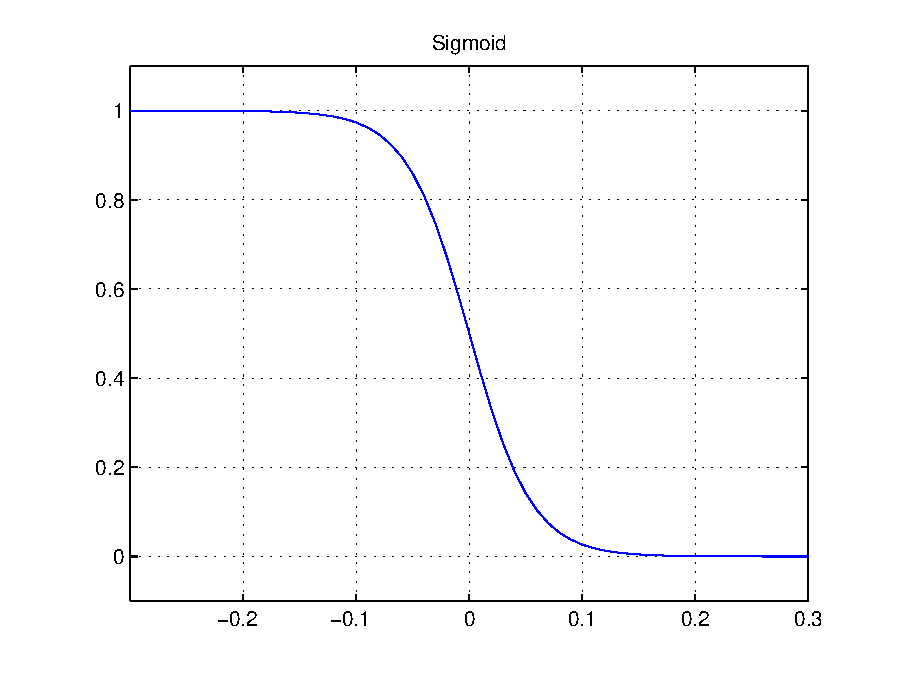
\includegraphics[scale=0.6]{./Pictures/sigmoid.eps}
\caption{SIGMOID 函数图像\label{fig:sigmoid}}
\end{figure}

或者也可以是$tanh$函数,其取值域为 $[-1,1]$,其表达式和函数图像为:
\begin{equation}
	f(x)=\frac{1-e^{-x}}{1+e^{-x}}
\end{equation}
\begin{figure}[H]
\centering
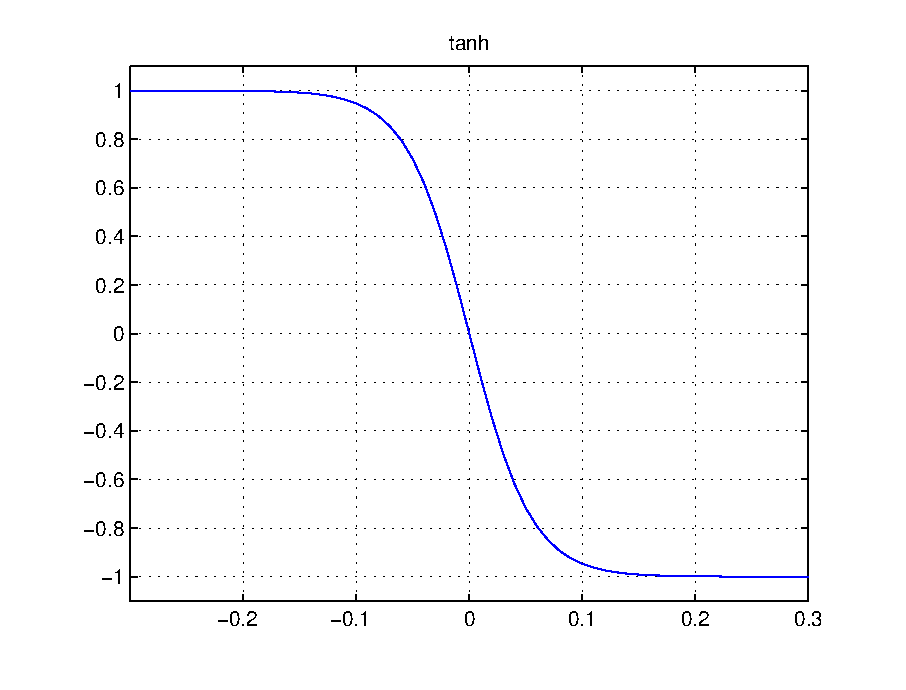
\includegraphics[scale=0.6]{./Pictures/tanh.eps}
\caption{TANH 函数图像\label{fig:tanh}}
\end{figure}


这类函数糅合了线性和非线性特性函数,当 $x$ 较大时函数迅速收敛至值域的边界,当 $x$ 较小时函数是S型的非线性函数,相比于传统的阈值函数能更好地模拟神经元的工作原理。

在解码阶段,映射函数 $g(h)$ 将隐含层特征空间映射回重构的输入层$\hat x$ ,表示为:
\begin{equation}
	\hat x=g(\hat{W}h+\hat b)
\end{equation}	
其中, $\hat{W}$ 为从隐藏层到输出层的权重矩阵,$h$为隐藏层矩阵,$\hat b$为隐藏层截距项, $g$ 是解码器的激活函数,若采用线性函数($g(x)=wx+b$),则该解码器被称为``线性解码器''(Linear Decoder),若采用$sigmoid$ 函数,则是原型自动编码器采用的架构。在训练自动编码器的过程中,我们利用迭代求解当前状态的梯度值,最终求得在训练样本集 $D$ 上一组最佳的参数配置 $\theta=\{W,\hat W,b,\hat b\}$ ,使系统的重构误差函数最小,重构误差函数的表达式为:
\begin{equation}
	J_{AE}=\sum\limits_{x_i \in D}L(x_i,g(f(x_i)))
\end{equation}
其中, $L$ 为每个输入项 $x_i$ 的重构误差值,一般地,我们使用平方误差函数或者交叉熵损失函数表示,二者数学公式分别表示为:
\begin{equation}\begin{array}{l}
	L(x,y)=\sum\limits_{x_i \in D}\|x_i-\hat x_i\|^2  \\
    L(x,y)=-\sum\limits_{x_i \in D}[x_i \ln \hat x_i+(1-x_i)\ln(1-\hat x_i)]
\end{array}\end{equation}
其中$\hat x_i=g(h(x_i))$,当我们采用$g$为线性函数时,系统的重构误差函数须采用平方误差函数。当我们采用$g$为 sigmoid函数时,系统的重构误差函数须采用交叉熵误差函数,这两者之间相互一一对应 \cite{17}。



图\ref{fig:origAE} 展示了原型自动编码器的结构。原型自动编码器包含输入层、隐藏层和输出层,其中编码过程对应于输入层到隐藏层的映射,解码过程对应于隐藏层到输出层的映射。

\begin{figure}[H]
\centering
\includegraphics[scale=0.4]{./Pictures/origAE.eps}
\caption{原型自动编码器模型}
\label{fig:origAE}
\end{figure}


\section{稀疏惩罚因子种类}
参数稀疏化的优点主要是:特征选择(Feature Selection)、可解释性(Interpretability)\cite{DBLP:journals/jmlr/Hoyer04}。稀疏规则化算子的引入能自动选择特征,去掉没有信息价值的特征点,即把这些特征对应的权重重置为0。只有少数特征对最终的决策其作用,有助于分析决策过程。

通过对原型自动编码器的隐藏层添加约束条件,使得绝大部分节点的数值接近0,我们能在隐藏层中获得原始数据的结构性特征\cite{wright2014sparse}。假设自定编码器的输入为$x$,我们的约束项为$\rho$,隐藏层神经元节点的平均激活度记作$\rho_j$。一般地,我们期望我们隐藏层的绝大多数神经元的取值在0 附近,少数神经元节点取值接近1,即只有少数神经节点处于激活状态。我们期望$\rho$取值在0附近(例如,0.05),同时令$\frac{1}{m}\sum_j^m{\rho_j}=\rho$。在稀疏自动编码器中,我们在模型的代价函数中增加稀疏惩罚项$KL(\rho||\rho_j)$,其表达式为:
\begin{equation}
	KL(\rho||\rho_j)=\rho \ln \frac{\rho}{\rho_j} + (1-\rho)\ln \frac{1-\rho}{1-\rho_j}
\end{equation}
此时,系统的代价函数为:
\begin{equation}
	J_{SAE}(W,b)=J(W,b)+\beta \sum_{j=1}^{s_2}KL(\rho||\rho_j)
\end{equation}
其中,$J_{SAE}(W,b)$代表稀疏自动编码器的代价函数,$J(W,b)$代表原型自动编码器的代价函数,$\beta$表示稀疏惩罚项的权重,$s_2$代表隐藏层节点个数\cite{24}。



\subsection{KL差分因子}
在概率论和信息论中,Kullback-Leibler差异(Kullback-Leibler Divergence)或简称KL距离,又称作相对熵(Relative Entropy),是衡量相同事件空间里面两个概率分布相对差距的测度\cite{DBLP:books/daglib/0016248,DBLP:conf/nips/BagnellB08}。在信息论中物理意义为度量使用基于$q(x)$的编码来编码来自$p(x)$的样本平均所需的额外的比特个数。两个概率分布$p(x)$和$q(x)$的相对熵定义为:
\begin{equation}
	D(p\|q)=\sum\limits_{x\in X}{p(x)\ln\frac{p(x)}{q(x)}};
\end{equation}
其含义是用概率分布 $q(x)$ 来近似概率分布 $p(x)$ 时丢失的信息。其中,$p(x)$是真实数据的分布,或者理论数据分布。$q(x)$ 是模型的预测分布,是对$p(x)$ 的一个近似估计。
该定义中约定$0\log (0/q)=0,p\log (p/0)=\infty$。若$p(x),q(x)$是连续分布的概率模型,那么其 KL-Divergence 定义为:
\begin{equation}
	D_{\mathrm{KL}}(p\|q) = \int_{-\infty}^\infty p(x) \, \ln\frac{p(x)}{q(x)};
\end{equation}
显然,当两个随机分布完全相同时,即$p=q$,其相对熵为0。当两个随机分布的差别增加时,其相对熵期望值也增大。图表\ref{fig:kl-divergence} 表明,该测量函数是非对称的函数,即 $D_{KL}(p\|q) \ne D_{KL}(q\|p)$, 从分布 $p$ 到 $q$ 的距离通常并不等于从 $q$ 到 $p$ 的距离。
\begin{figure}[H]
\centering
\includegraphics[scale=0.2]{./Pictures/kl.eps}
\caption{KL差异因子的函数图像}
\label{fig:kl-divergence}
\end{figure}



\subsection{L1范数因子}
L1范数也叫``稀疏规则算子(Lasso Regularization)'',是指向量中各个元素绝对值之和。它是L0范数的最优凸近似\cite{DBLP:conf/cvpr/YangYGH09}。L0范数指的是向量中非0元素的个数。如果我们用L0范数来规则化参数矩阵W的话,就是希望W的大部分元素都是0.换句话说,就是让参数W是稀疏的。由于L0范数很难求解(NP难问题),相对的L1范数更易求解,所以在一定条件下,求解L0 范数以概率1意义下等价于L1范数:
\begin{equation}
\left\{ \begin{array}{l}
\min \|x\|_0 \\
s.t.Ax = b
\end{array} \right. \Rightarrow \left\{ \begin{array}{l}
\min \|x\|_1 \\
s.t.Ax = b
\end{array} \right.
\end{equation}
所以,L1范数和L0范数可以实现稀疏,L1因具有比L0更好的优化求解特性而被广泛应用。

实验中使用的L1范数计算公式为:
\begin{equation}
S_{L1}=\sum\limits_{i=1}^{n}{|h_{\theta}(x^{(i)})|};
\end{equation}
由于L1范数在0处不可导\cite{DBLP:conf/nips/LeeBRN06},为了便于计算,我们采用近似公式来计算其L1范数\cite{DBLP:journals/corr/abs-1005-4717}:
\begin{equation}
S_{L1}=\sum\limits_{i=1}^{n}{|h_{\theta}(\sqrt{x_i^2+\varepsilon})|},\varepsilon =1e-4;
\end{equation}

\subsection{L2范数因子}
除了L1范数,还有一种更优的规则化范数是L2范数:$\|W\|_2$。其效果也不逊于L1范数,在回归算法中被称作``岭回归(Ridge Regression)'',也被称作``权值衰减项(Weight decay)'' \cite{yang2011robust}。其强大功效是改善机器学习中的过拟合问题。过拟合问题指的是模型训练时误差很小,但是在测试时误差很大,即模型复杂到可以拟合到我们所有的训练样本了,但对新的测试样例无法做出正确的决策。

L2范数指的是像两个元素的平方和然后求平方根。我们让$\|W\|_2$最小化,可以使得$W$的每个元素都很小,接近于0。实际上有效地限制了多项式分量对系统的影响,在一定条件下避免了过拟合的出现,提升模型的泛化能力。实验中使用的L2范数计算公式为:
\begin{equation}
S_{L2}=\sum\limits_{i=1}^{n}{h_{\theta}(x^{(i)})^2};
\end{equation}



\subsection{Student-t惩罚因子}
\begin{defn}[正态分布]
	若随机变量 $X$ 服从一个均值为 $\mu$ 、方差为 $\sigma$ 的概率分布,其概率密度函数为:
	\begin{equation}
	f(x)=\frac{1}{\sqrt{2\pi}\sigma}\exp\left(-\frac{(x-\mu)^2}{2\sigma^2}\right)
	\end{equation}
	则这个随机变量服从正态分布,记作 $X\sim N(\mu,\sigma^2)$。
\end{defn}
\begin{defn}[标准正态分布]
	当 $\mu=0,\sigma=1$ 时,正态分布就成为标准正态分布
	\begin{equation}
	f(x)=\frac{1}{\sqrt{2\pi}}\exp\left(-\frac{x^2}{2}\right)
	\end{equation}
\end{defn}
正态分布(Normal Distribution)是许多统计方法的理论基础。由于在实际工作中,往往 $\sigma$未知,故我们常用样本标准差 $s$ 作为 $\sigma$ 的估计值,成为:
\begin{equation}
	t=\frac{\overline x-\mu}{s/\sqrt{n}}
\end{equation}
其中 $n$ 为样本数量,$\overline x$为样本平均值($\overline x=(x_1+x_2+\cdots+x_n)/n$),$s$为样本标准差($s=\frac{1}{n-1}\sum\limits_{i=1}^n{(x_i-\overline {x_n})^2}$),$\mu$ 为总体平均值。由于样本标准差随着抽样手段而波动,于是在用 $s$ 代替 $\sigma$ 后,上式便不呈正态分布而呈t分布。

Student-t 统计概率分布模型由 William Gosset 在1908年发表\cite{DBLP:conf/nips/WellingHO02},其的概率分布函数为:
\begin{equation}
	f(x)=\frac{\Gamma(\frac{n+1}{2})}{\sqrt{n\pi}\Gamma(\frac{n}{2})}(1+\frac{x^2}{n})^{\frac{n+1}{2}};
\end{equation}
参数 $n$ 称为 t 分布的自由度, $\Gamma(n/2)$ 是参数为 $n/2$ 的 $\Gamma$ 函数:
\begin{equation}
	\Gamma(r)=\int_0^\infty{x^{r-1}e^{-x}dx},(r>0);
\end{equation}

实验中选择其简单形式的函数$S_{student}(x)$ :
\begin{equation}
S_{student}(x)=\sum\limits_{i=1}^{n}{log(1+h_{\theta}^2(x^{(i)}))};
\end{equation}
其一阶导数 $S'_{student}(x)$为:
\begin{equation}
S'_{student}(x)=\frac{2x}{1+x^2};
\end{equation}
其数学函数和其一阶导数图像,如图\ref{fig:t},\ref{fig:dt}所示。
\begin{figure}[H]
\centering
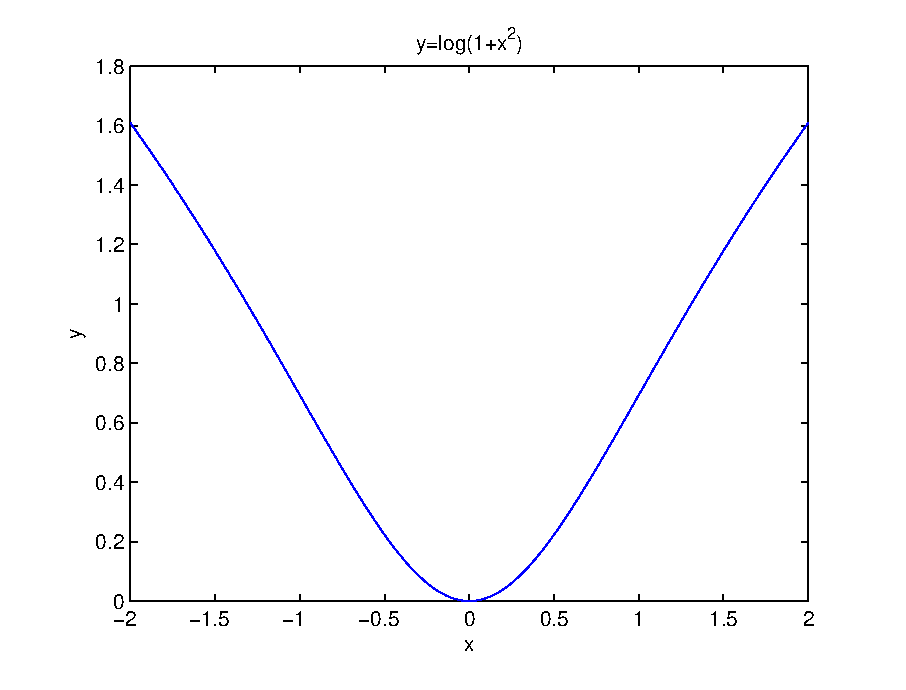
\includegraphics[scale=0.5]{./Pictures/t.eps}
\caption{STUDENT-T 因子的函数图像}
\label{fig:t}
\end{figure}

\begin{figure}[H]
\centering
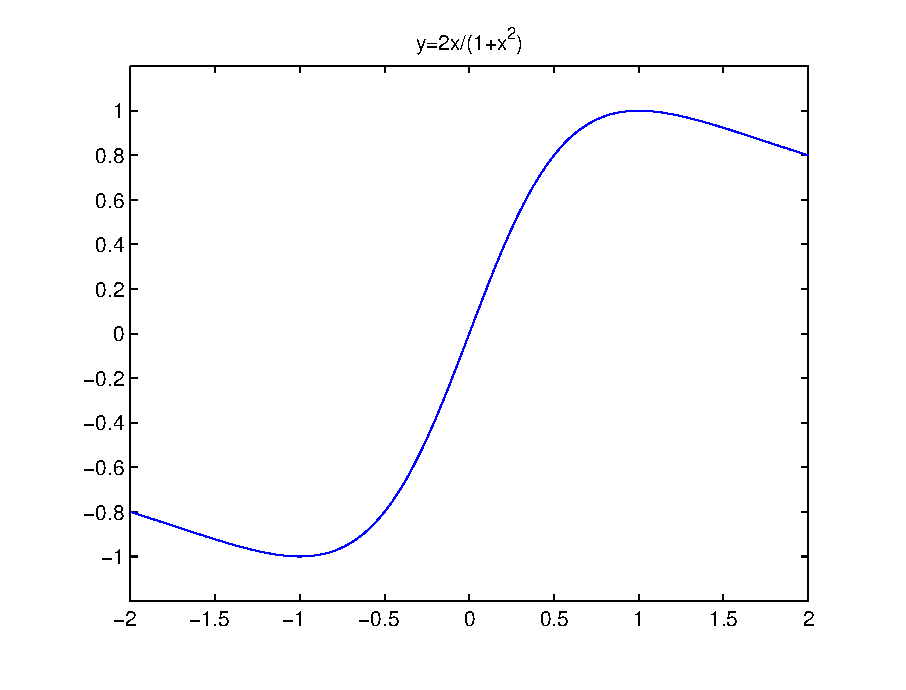
\includegraphics[scale=0.5]{./Pictures/pt.eps}
\caption{STUDENT-T 因子函数一阶导数图像}
\label{fig:dt}
\end{figure}


\section{Softmax分类器模型}
传统的logistic回归模型只能适用于二元分类模型,类标签$y$只能取两个值($y=\{0,1\}$),无法解决多元分类问题。在原有基础上,推导出的Softmax回归模型能解决多元分类问题,类标签$y$能选择多个值($y=\{0,1,\cdots,n\}$)\cite{Krizhevsky2012ImageNet}。Softmax回归模型能有效识别手写数字分类问题,例如MNIST数据集上的数字识别问题,辨识10个不同的单个数字。我们也来用梯度下降算法来训练Softmax回归模型$J(\theta;\lambda)$,但在训练该模型的同时,我们还需要通过K层交叉验证手段配置合适的超参数$\lambda$,以获得最优的模型参数配置。其计算公式如下所示:

\begin{equation}
\label{equ:softmax}
{h_\theta }({x^{(i)}}) =  \arg\max\limits_{k} \left[ {\begin{array}{*{20}{c}}
{p({y^{(i)}} = 1|{x^{(i)}};\theta )}\\
{p({y^{(i)}} = 2|{x^{(i)}};\theta )}\\
 \dots \\
{p({y^{(i)}} = k|{x^{(i)}};\theta )} \\
 \dots \\
{p({y^{(i)}} = K|{x^{(i)}};\theta )} \\
\end{array}} \right]=\arg\max\limits_{k} \frac{1}{\sum\limits_{j=1}^{K}{e^{\theta_j^Tx^{(i)}}}}\left[ {\begin{array}{*{20}{c}}
{e^{\theta_1^Tx^{(i)}}}\\
{e^{\theta_2^Tx^{(i)}}}\\
 \dots \\
{e^{\theta_k^Tx^{(i)}}}\\
 \dots \\
{e^{\theta_K^Tx^{(i)}}}\\
\end{array}} \right]
\end{equation}
其中 $\theta_1, \theta_2, \ldots, \theta_k \in \Re^{n+1}$ 是模型的参数。请注意 $\frac{1}{ \sum_{j=1}^{k}{e^{ \theta_j^T x^{(i)} }} } $这一项对概率分布进行归一化,使得所有概率之和为 1 。


通过预训练手段我们获得了参数$\theta$,对于每一个测试样例$x^{(i)}$,我们计算该样例在符合类标签$k$的概率$p({y^{(i)}} = k|{x^{(i)}};\theta )$,其中类标签$k \in \{1,2,\dots,k,\dots,K\}$。通过选取最大概率的类标签,我们就确定了样例$x^{(i)}$所匹配的$y^{(i)}$。训练过程中,系统的代价函数为:
\begin{equation}
	J(x;\theta)=\sum\limits_{i=1}^{n}{\|h_{\theta}(x^{i})-y^i\|^2};
\end{equation}



\section{迭代优化函数选取}
拟牛顿法(Quasi-Newton Methods)能有效求解非线性优化问题,由20世纪50年代由美国 Argonne 国家实验室的W.V.Davidon 提出的。不久,R.Fletcher和M.J.D.Powell证明这种算法远比传统方法快速可靠,使得非线性优化这门学科在这之后突飞猛进。在之后的20年里,拟牛顿方法出现了大量的变形公式以及是以百计的相关论文\cite{陈姗2013求解无约束最优化问题的一个新的拟牛顿方法}。DFP方法、BFGS方法以及L-BFGS算法都是重要的拟牛顿法。先介绍什么是牛顿法,为此,考虑如下无约束的极小化问题:
\begin{equation}
	\label{equ:mins}
	\min_{x}{f(x)},x=(x_1,x_2,\dots,x_N )^T \in R^N 
\end{equation}
假定$f$为凸函数,且两阶连续可微。此外记极小问题\ref{equ:mins}的解为$x^*$。
\subsection{牛顿法}
牛顿法的基本思想是:在现有极小点估计值附近对$f(x)$做二阶泰勒展开,进而找到极小点的下一个估计值。设$x_k$为当前极小点估计值,则:
\begin{equation}
	\phi(x)=f(x_k )+f'(x_k )(x-x_k )+\frac{1}{2}f''(x_k )(x-x_k )^2
\end{equation}
表示$f(x)$在$x_k$附近二阶泰勒展开式(略去了关于$x-x_k $的高阶项)。由于求的是极值,故令:$\phi '(x)=0$,解得:
\begin{equation}
	x=x_k +\frac{f'(x_k )}{f''(x_k )},
\end{equation}
给定初始值$x_0 $,则可以构造如下的迭代格式:
\begin{equation}
	x_{k+1 }=x_k +\frac{f'(x_k )}{f''(x_k )},k=0,1,\dots
\end{equation}
产生的序列$\{x_k \}$来逼近$f(x)$的极小点。在一定条件下,$\{x_k \}$可以收敛到$f(x)$的极小点。

若目标函数是二阶函数,由于二阶函数泰勒展开与原目标函数是完全相同的二次式,海森矩阵退化成一个常数矩阵,从任意初始点出发,只需一步迭代就可以达到$f(x)$的极小点$x^*$,因此对于非二次函数,若函数的二次性态较强,则其的收敛速度也是很快的,这是牛顿法的主要优点。但原始牛顿法由于迭代公式中采用的是定长迭代,对于非二次型目标函数,有时会使目标函数值上升,即出现$f(x_{k+1 }>f(x_k ))$情况,这表明原始牛顿法不能保证函数值稳定地下降,在特殊情况下甚至可能造成迭代点列$\{x_k\}$的发散,从而无法计算其最优解。
\subsection{拟牛顿方法}
拟牛顿方法的基本思想是:不用二阶偏导函数而构造出可以近似海森矩阵的正定对称阵,在``拟牛顿''的条件下优化函数。不同的构造方法就产生了不同的拟牛顿方法。BFGS算法是Broyden,Fletcher,Goldfarb,Shanno四位优化大家在1970年几乎同时从不同的优化角度提出的。时至今日,它仍然被认为是最好的拟牛顿算法。但是该方法的矩阵存储量为$n^2$ ,因此维度很大时内存不可接受。同时,矩阵非稀疏会导致训练速度慢。针对BFGS的缺点,L-BFGS的基本思想是只保存最近的m次迭代信息,从而大大降低数据存储空间 。

本实验对稀疏自动编码器和Softmax分类器的系统代价函数参数优化阶段采用L-BFGS算法\cite{nocedal1980updating,liu1989limited}。其流程步骤如图所示。
\begin{figure}[H]
\centering
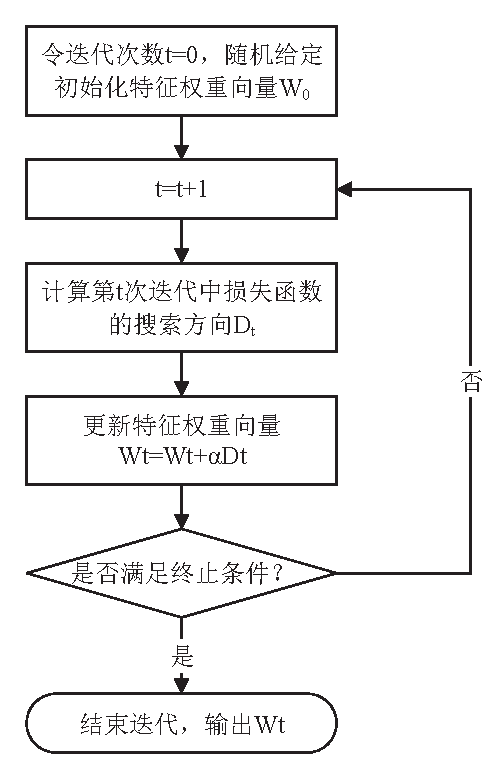
\includegraphics[scale=0.7]{./Pictures/optimize.eps}
\caption{优化方法的基本步骤\label{fig:framework}}
\end{figure}
对于参数矩阵的初始化问题,我们采用均匀分布模型对其进行随机初始化操作。记每一层的权重参数矩阵为$W^l$,则:
\begin{equation}
  -\sqrt{\frac{6}{(fan_{in} + fan_{out})}} \le W^l \le \sqrt{\frac{6}{(fan_{in} + fan_{out})}}
\end{equation}
其中 $fan_{in}$是该层神经网络输入节点数量,$fan_{out}$是该层神经网络输出节点数量\cite{张娇2011基于}。

MATLAB中调用优化函数的方式为:
\begin{minted}[mathescape,
               linenos,
               numbersep=5pt,
               gobble=2,
               frame=lines,
               framesep=2mm]{MATLAB}
    addpath minFunc;
    opttheta = theta; 
    options.Method = 'lbfgs';
    options.display = 'on';
    [opttheta, cost] = minFunc( @(p) sparseAutoencoderCost(p, ...
                                   inputSize, hiddenSize, ...
                                   lambda, sparsityParam, ...
                                   beta, unlabeledData,...
                                   gamma,epsilon), ...
                                   opttheta, options);
\end{minted}
首先将优化函数的路径``minFunc''添加至MATLAB环境中,其次配置优化函数为``L-BFGS'',最大的迭代次数为400次,最后将自动编码器的代价函数以参数形式传给minFunc函数,最后该函数会返回最优化的opttheta。

\section{交叉验证手段}
交叉验证(Cross-Validation)主要用于PCR 、PLS 回归建模中,目的是减小模型的泛化误差。在给定的数据样本中,可以使用60\% 数量的样本作为训练集进行建模,留20\%数量的样本检测用刚建立的模型,并记录它们的平方加和。每个样本的交叉验证误差平方和称为PRESS(Predicted Error Sum of Squares)。

它能有效防止训练模型的过拟合问题,获得更稳定的模型。常用的精度测试方法主要是K折交叉验证,这个方法的优势在于,同时重复运用随机产生的子样本进行训练和验证,每次的结果验证一次,通常选择 $k=10$。



\section{实验性能评价指标}
\subsection{稀疏度}
我们使用以下函数计算特征的稀疏度,以评价不同自动编码器生成稀疏特征的性能 \cite{DBLP:journals/jmlr/Hoyer04}。
\begin{equation}
sparseness(\textbf{x}) = \frac{\sqrt{N} - (\sum_i{|x_i|}) / \sqrt{\sum_i{x_i^2}}}{\sqrt{N} - 1}
\end{equation}
其中,n是特征向量的维度。只有当 x只剩下一个非零值时,该函数才会取值为1;若是所有值取值相同,该函数取值为0.即,函数取值为1时,特征x将会十分稀疏。若是特征取值为0,则特征的稀疏性很差。

\subsection{重构误差}
重构误差的计算公式为:
\begin{equation}
	reconstruction_error(x)=\frac{1}{n}\sum\limits_{i=1}^{n}{\|x-\hat x\|^2};
\end{equation}
其中$\hat x=g(W'h(Wx+b)+b')$是稀疏自动编码器所重构出来的输入值,通过统计输入值与重构的输入值的大小,来描述该编码器的泛化误差,泛化误差越小,说明自动编码器学习的特征越有效。

\subsection{测试集正确率}
测试过程中,我们通过统计模型的预测标签与真实标签是否匹配来确定系统的正确率,其计算函数为:
\begin{equation}
	accuracy(x;\theta)=\sum\limits_{i=1}^{n}{\frac{h_{\theta}(x^{(i)})==y^{(i)}}{n}}
\end{equation}
其中$y^{(i)}$是测试样例的正确类标签,$h_{\theta}(x^{(i)})$是Softmax分类器的预测类标签。

\section{本章小结}
本章讲述了算法流程的基本步骤,下图是实验算法的模型框架图:
\begin{figure}[H]
\centering
\includegraphics[scale=0.4]{./Pictures/framework.eps}
\caption{实验研究的基本框架\label{fig:framework}}
\end{figure}

实验框架如图\ref{fig:framework}所示,主要由4个部分组成:数据预处理、稀疏自编码器训练、Softmax回归模型训练、统计计算实验指标。当我们利用训练数据集完成了稀疏自编码器和Softmax回归模型的训练后,我们将采用测试数据集,按顺序输入稀疏自编码器和Softmax回归模型,与此同时我们需要统计:稀疏自编码器中获得的特征稀疏度、稀疏自编码器在测试集上的平均重构误差、Softmax模型的识别准确率。我们拟采用五个图像数据集,分别输入模型,再收集不同数据集上的数据后,分析其性能表现。


\chapter{实验平台设计}
\section{功能模块设计}
主要的功能模块分为:展示任务运行状况、提交计算任务、展示实验计算结果,如下图\ref{fig:module}所示。
\begin{figure}[H]
\centering
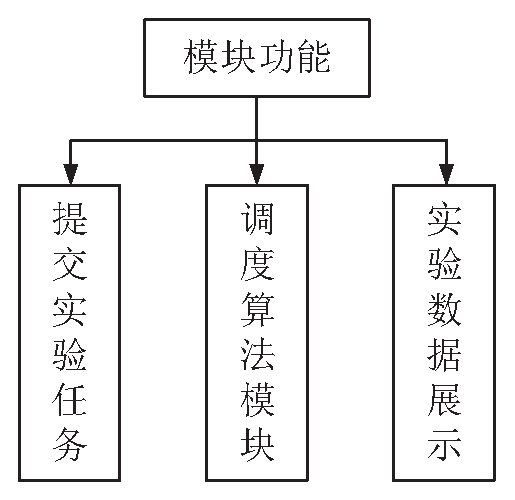
\includegraphics[scale=0.5]{./Pictures/module.eps}
\caption{系统功能模块}
\label{fig:module}
\end{figure}


\section{数据表设计与实现}
本实验平台主要任务是管理用户提交的计算任务,故需要建立相应的数据表。为了方便管理,我们需要用户提供其用户名,本次计算任务的任务名还有相应的测试集和训练集,最后系统添加上提交任务的时间,一旦人物运行中出现差错,这些信息也方便管理员追踪检查错误源,排查问题。
\begin{table*}[H]
\begin{center}
{
\caption{DJANGO中定义的数据表设计}}
\begin{tabular}{|c|c|c|c|c|c|}
\hline
字段& 类型&含义\\
\hline
taskname &charfield(max-length(200)) &任务名\\
\hline
username &charfield(max-length(200)) &  用户名\\
\hline
pub-date & DateField()& 任务提交时间\\
\hline
trainingFile  & FileField() &  训练集文件\\
\hline
testFile & FileField() &  测试集文件\\
\hline
status &Charfield() & 任务运行状态\\
\hline
tasknote  & textfield() & 提交任务时的注记 \\
\hline
\end{tabular}
\end{center}
\end{table*}



\subsection{前台设计}
为了展示实验结果,同时便于实验配置与操作,故设计了基于django架构\footnote{Django: www.djangoproject.com}的实验配置平台。该平台主要完成实验计算任务提交,实验数据结果展示功能和实验进度显示功能。由于针对部分较大的实验数据集,训练时间需要数百小时,若简单的采用MATLAB软件的GUI图形界面会导致界面卡死,长时间不响应等现象,无法满足人机交互准则。在计算任务提交环节,需要用户提交实验训练集和实验测试集,并自行指定数据预处理方法。由于针对不同数据源,数据预处理的优良对实验结果影响非常大,故采用单一的无法满足实验要求,故平台给出一系列预处理方法以供用户选择。实验数据结果展示页面主要展示MATLAB实验保存的实验图表,平台按照任务分类展示在界面上,用户也可以下载压缩实验数据图表资源,以供用户分析实验数据。实验进度显示界面主要展示不同任务的运行情况,以及当前系统的CPU,内存占用情况。

另一方面,考虑到界面设计的美观大方,采用时下流行的 Bootstrap 技术,选取 BeyondAdmin 模板作为Django框架的网页开发的静态模板。在静态模板中添加django框架的动态编程语言,完成系统所需的功能需求。

第一个界面是统计用户提交的计算任务,以表格的形式展示用户的任务是否正在运行(In Progress),或者遇到什么错误(Issued),或者已经成功结束运算(Finished)。若是遇到什么问题,需要管理员在后台查询错误原因,将信息反馈给用户。
\begin{figure}[H]
\centering
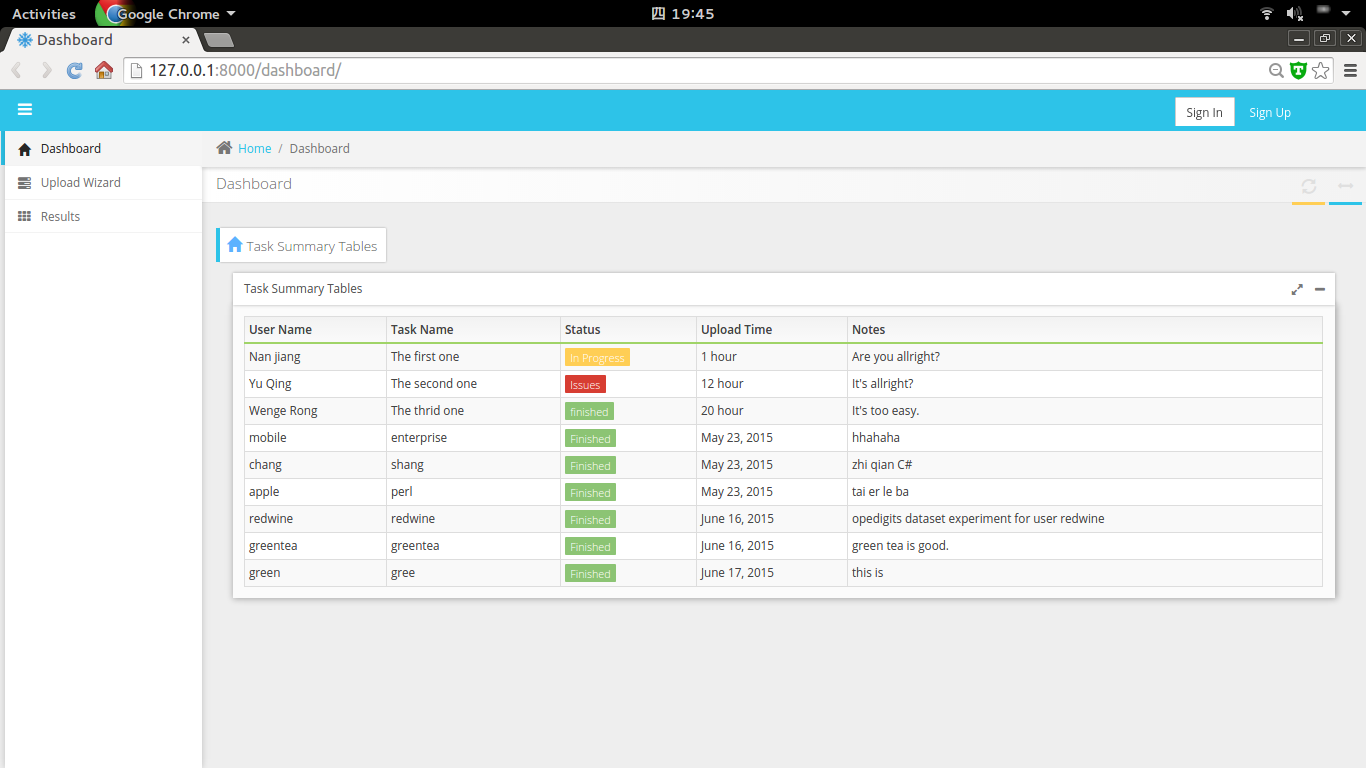
\includegraphics[width=0.7\linewidth]{./Pictures/django01.png}
\caption{任务统计界面\label{fig:framework}}
\end{figure}

第二个界面是用户提交计算任务界面,用户填写任务名称和提交训练集和测试集,与此同时,用户可以选择数据集数初始化手段。针对不同的需要合理选择预处理手段,将此功能给用户选择,以便提高实验成功率。最后用户也可以选择填写一些实验注记,以便管理员维护。
\begin{figure}[H]
\centering
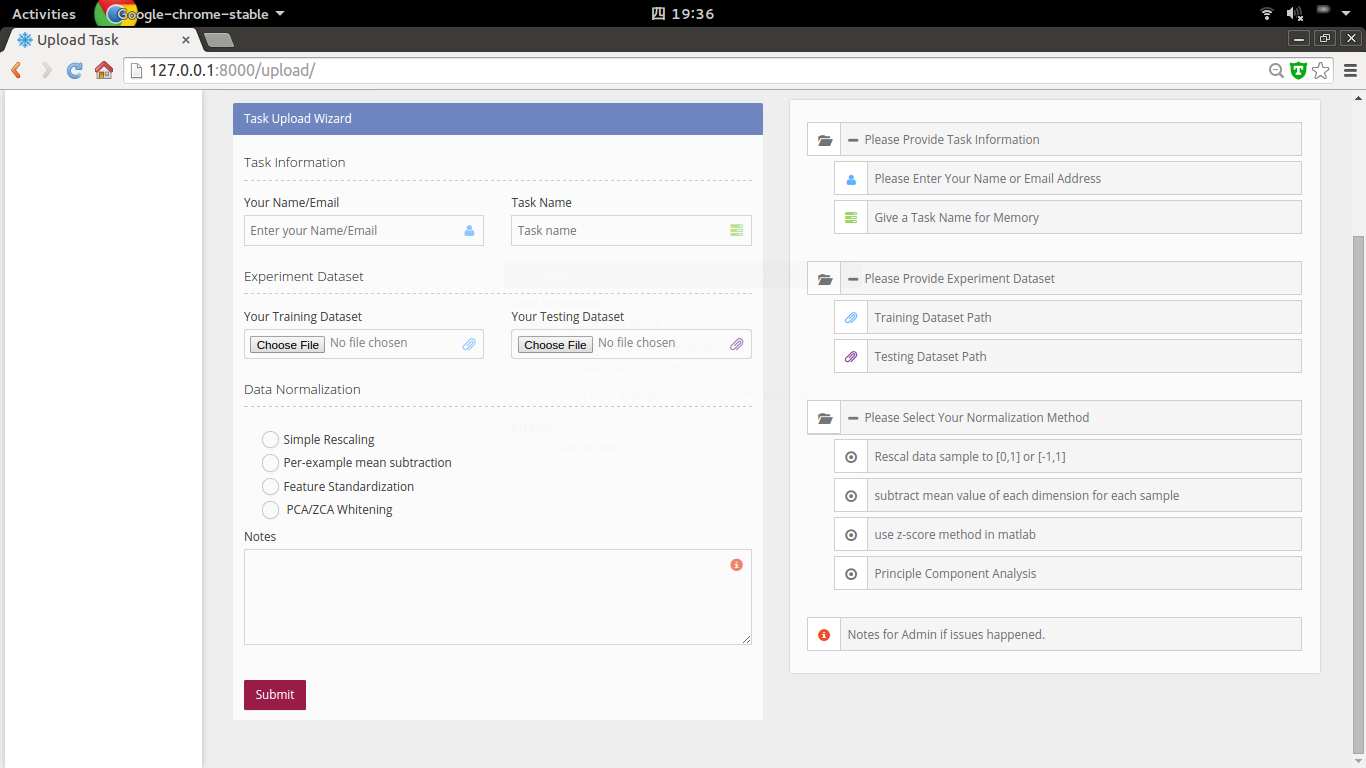
\includegraphics[width=0.7\linewidth]{./Pictures/django02.png}
\caption{任务提交界面\label{fig:framework}}
\end{figure}

最后一个界面是展示实验运算准确率,主要分为两张图表,一张是分类正确率随着稀疏参数变化的图表,另一张是特征稀疏度随着稀疏参数的变化的图表。
\begin{figure}[H]
\centering
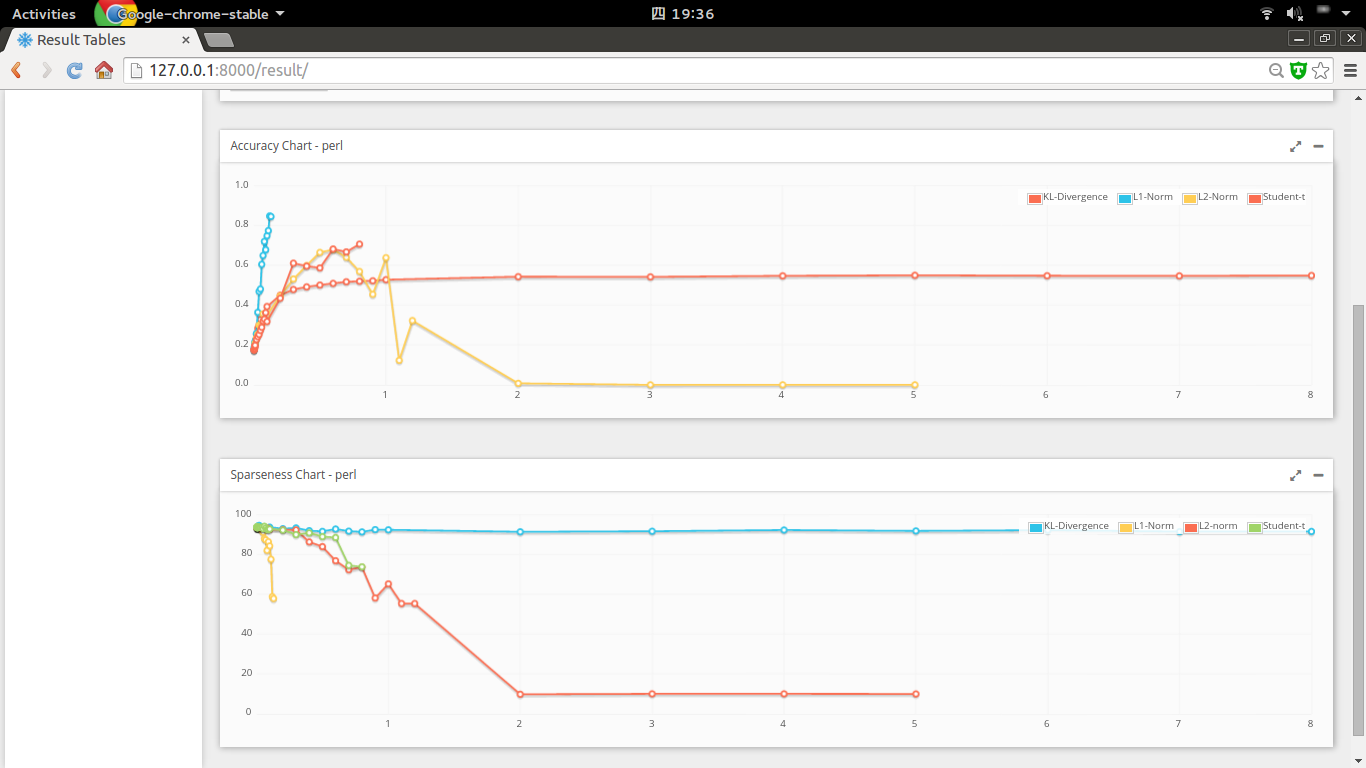
\includegraphics[width=0.7\linewidth]{./Pictures/django03.png}
\caption{任务结果展示界面\label{fig:framework}}
\end{figure}


\subsection{接口函数设计与实现}
为了便于在python中调用MATLAB算法模块,我们采用command-line的形式调用,同时我们需要MATLAB算法运行在后台程序,故同时也需要使用linux的nohup指令。在应用Unix/Linux时,我们一般想让某个程序在后台运行,于是我们将常会用$\&$在程序的结尾让程序自动后台运行。可是一旦我们注销或者屏保后,这个脚本程序就会被自动停止,这是我们需要nohup指令。
\begin{minted}[mathescape,
               linenos,
               numbersep=5pt,
               gobble=2,
               frame=lines,
               framesep=2mm]{Shell}
    nohup MATLAB -nodisplay -nodesktop < script.m >run.log 2>run.err & 
\end{minted}

其中 $<$是输入重定向符号,$>$是输出重定向符号,$2>$是错误重定向符号。这里我们新建一个MATLAB脚本文件script.m,将测试集和训练集和目录写入,调用 MATLAB 算法模块,接着将这个script.m文件作为MATLAB系统的的默认输入文件,实现了后台自动调用MATLAB算法模块的功能,与此同时,为了记录程序运行时的状态,我们将MATLAB程序的正确与错误输出重定向到文件中,以便后续维护所用。


\chapter{实验结果与分析}
\section{实验采用的数据集}
\subsection{MNIST Handwritten Digits字符库}
MNIST字符库包含有60000张数字0~9训练样本数据集和10000张数字0~9的测试集,每张图片均为灰度图,取值域为 $[0,255]$\cite{lecun1998gradient}。它是NIST数据库的一个子集,这些数字图像已经被预处理和格式化,图像大小一致,数字位置一致。
\begin{figure}[H]
\centering
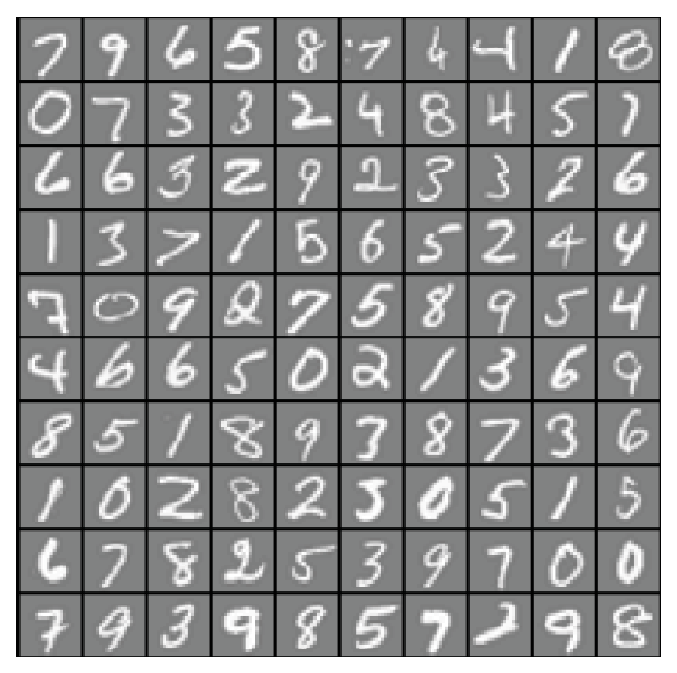
\includegraphics[scale=0.5]{./Pictures/mnist-icon.eps}
\caption{MNIST数据库样例\label{fig:mnist-icon}}
\end{figure}



\subsection{NORB物体识别数据库}
NORB数据库主要用于三维物体形状识别实验 \cite{DBLP:conf/cvpr/LeCunHB04}。它包含50个玩具属于5类形象:四肢动物,人像,飞机,卡车和汽车。物体采集是在两台相机,6种光照条件下获取的。采集角度是30度到70度,每隔5度,并且在18个方位(0到340每20度)分别采集图像。训练集是由5种类别组成(标号为4,6,7,8,9),测试集选用剩下的实例(标号为0,1,2,3,5)。

图像采集后,每张图片均已作预处理,物体对象已被放置在图像中心,缩放到统一的尺寸大小,并且图片的背景和阴影均统一。物体对象之间的差异主要为:光照变化、旋转角度、水平位移和垂直位移。
\begin{figure}[H]
\centering
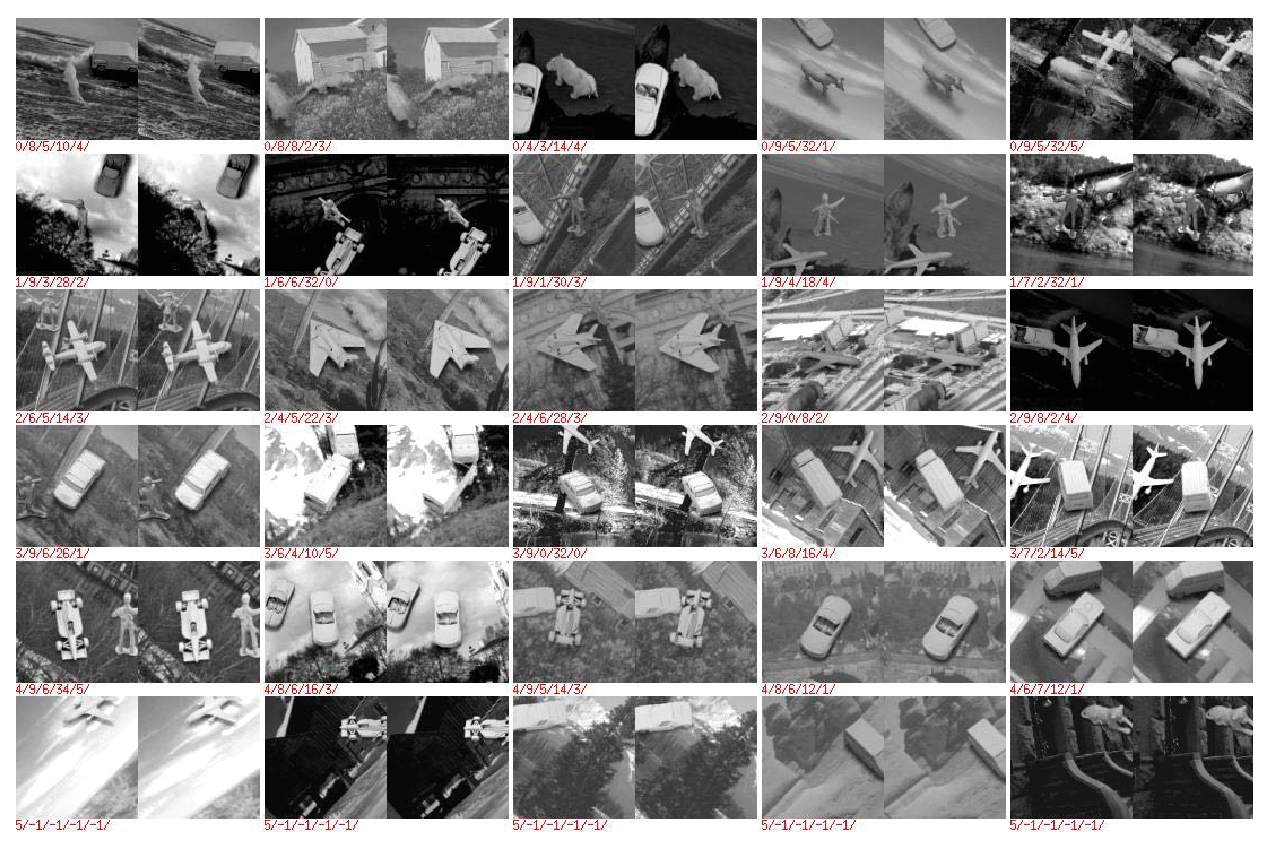
\includegraphics[scale=0.5]{./Pictures/norb-icon.eps}
\caption{NORB数据库样例\label{fig:norb-icon}}
\end{figure}

\subsection{SVHN街道房屋数字数据库}
SVHN数据集(The Street View House Numbers Dataset)是开发机器学习和数据预处理和格式要求最小的物体识别算法的真实世界的图像数据集\cite{netzer2011reading}。它和MNIST数据集的内容大致相似(例如,图像是小数字,但采用裁剪)级以上的标记数据的顺序(超过600000张图像),源于更加复杂的真实世界的案例(识别数字和数字的自然场景图像)。SVHN数据集采集自谷歌街景中房屋上面的数字。
\begin{figure}[H]
\centering
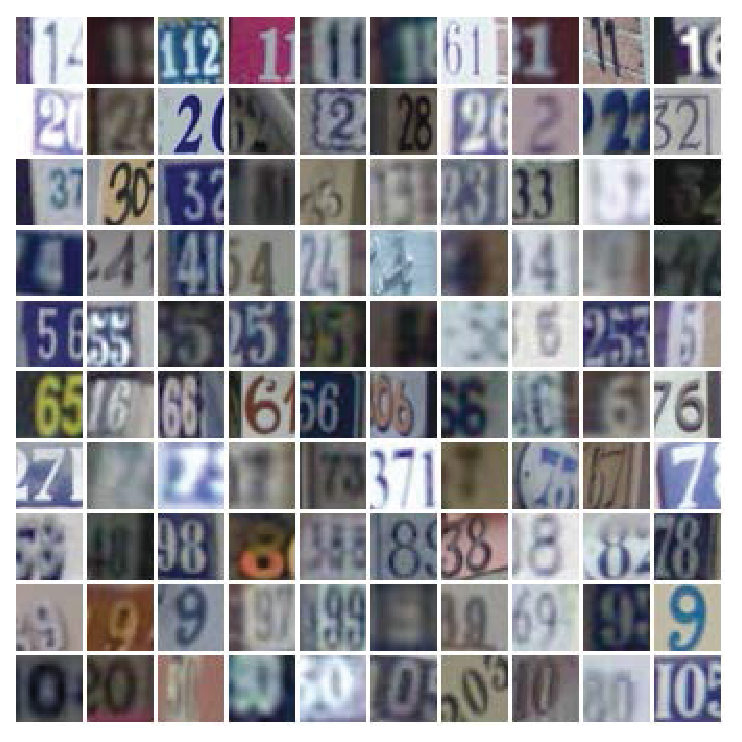
\includegraphics[scale=0.5]{./Pictures/svhn-icon.eps}
\caption{SVHN数据库样例\label{fig:svhn-icon}}
\end{figure}


\subsection{OPTDIGITS手写数字库}
OPTDIGITS数据库(Optical Recognition of Handwritten Digits Data Set)采集自43个人,其中的30人书写的数字作为训练集,剩下13人的数字作为测试集\cite{Bache+Lichman:2013}。每张图的大小为 32x32被划分为4x4的小块,每个 8x8的小块均代表一个数字,数字的范围为0-16。这样的低像素的数字图像能有效降低了参数维度,增加了模型对误差的鲁棒性。数据库已采用NIST的数据预处理工具做了规范化操作。
\begin{figure}[H]
\centering
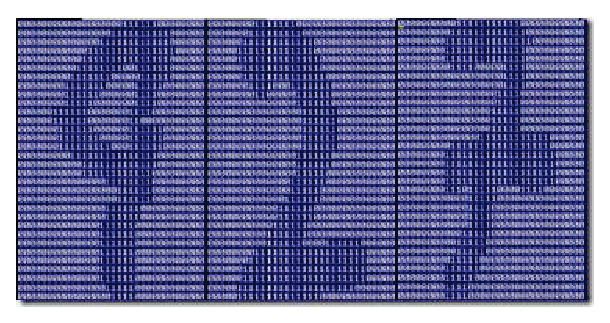
\includegraphics[scale=0.5]{./Pictures/optdigits-icon.eps}
\caption{OPTDIGITS数据库样例\label{fig:svhn-icon}}
\end{figure}



\subsection{CIFAR-10数据库}
CIFAR-10 数据库包含 32x32像素的60000张彩色图像,一共分为10个类,每个类别有6000张,分别包括:飞机、鸟类、猫、鹿、狗、青蛙、马、船、卡车和汽车\cite{krizhevsky2009learning}。这些类别是互相排斥的。汽车和卡车类别之间是没有交叉数据的。``汽车''‘包括轿车、越野车等等,``卡车''只包括大卡车,不包括皮卡。
\begin{figure}[h]
\centering
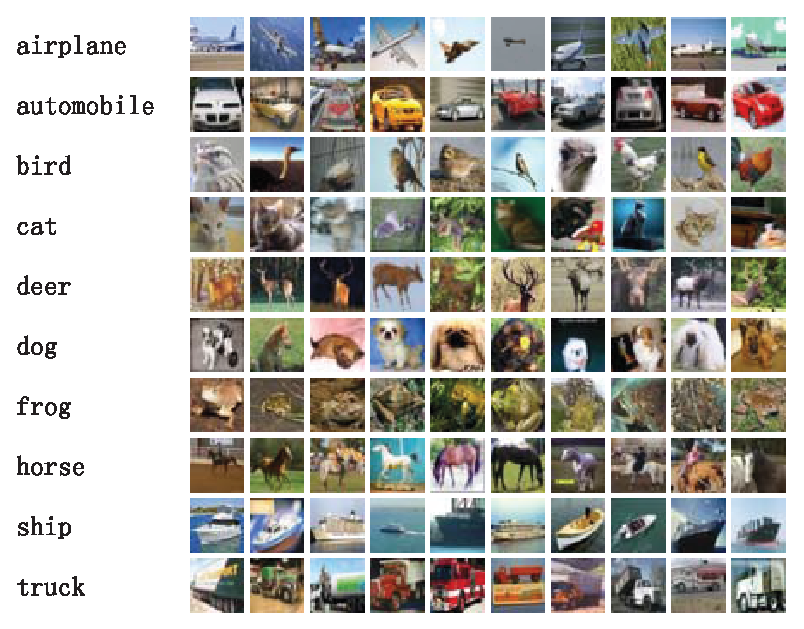
\includegraphics[scale=0.7]{./Pictures/cifar-icon.eps}
\caption{CIFAR-10数据库样例\label{fig:cifar-icon}}
\end{figure}

实验中对于五种数据集训练集需要划分出一部分作为交叉验证集,下表展示了总结数据。由于数据集测维度影响自动编码器输入层和隐藏层节点的数量,故同时给出自动编码器的配置数据。由于输出层节点数量始终等于输入层节点数量,故无需配置。
\begin{table}[h]
\begin{center}
{
\caption{数据集组成和稀疏自动编码器配置}\label{datasetconfig}}
\begin{tabular}{|c|c|c|c|c|c|}
\hline
数据集& 训练集&交叉验证集&测试集&输入层节点数量&隐藏节点数量\\
\hline
MNIST & 50,000 & 10,000 & 10,000 & 784 & 196 \\
\hline
CIFAR-10 & 45,000 & 5,000 & 10,000 & 3072 & 400 \\
\hline
SVHN  & 72,257 & 1,000 & 26,032 & 3072 & 500 \\
\hline
OPTDIGITS & 3,823 & 3,000 & 1,797 & 63 & 20 \\
\hline
NORB  & 23,300 & 1,000 & 23,300 & 6912 & 500 \\
\hline
\end{tabular}
\end{center}
\end{table}



\section{实验结果展示}
\subsection{特征可视化}
在展示实验结果之前,我们先将自动编码器训练获得的特征绘制成图像,以便分析特征有效性,这里以MNIST数据集为例。下图展示了纯自动编码器和配置不同稀疏因子的自动编码器学习到的特征。

\begin{figure}[h]  
\centering
\caption{自动编码器配置不同惩罚因子学习到的特征\label{fig:no}}  
\begin{minipage}[h]{0.8\linewidth}
\centering
\includegraphics[scale=0.5]{./figure/MNIST_No_penalty_weight.eps}
\end{minipage}
\hfill
\begin{minipage}[h]{0.8\linewidth}
\centering
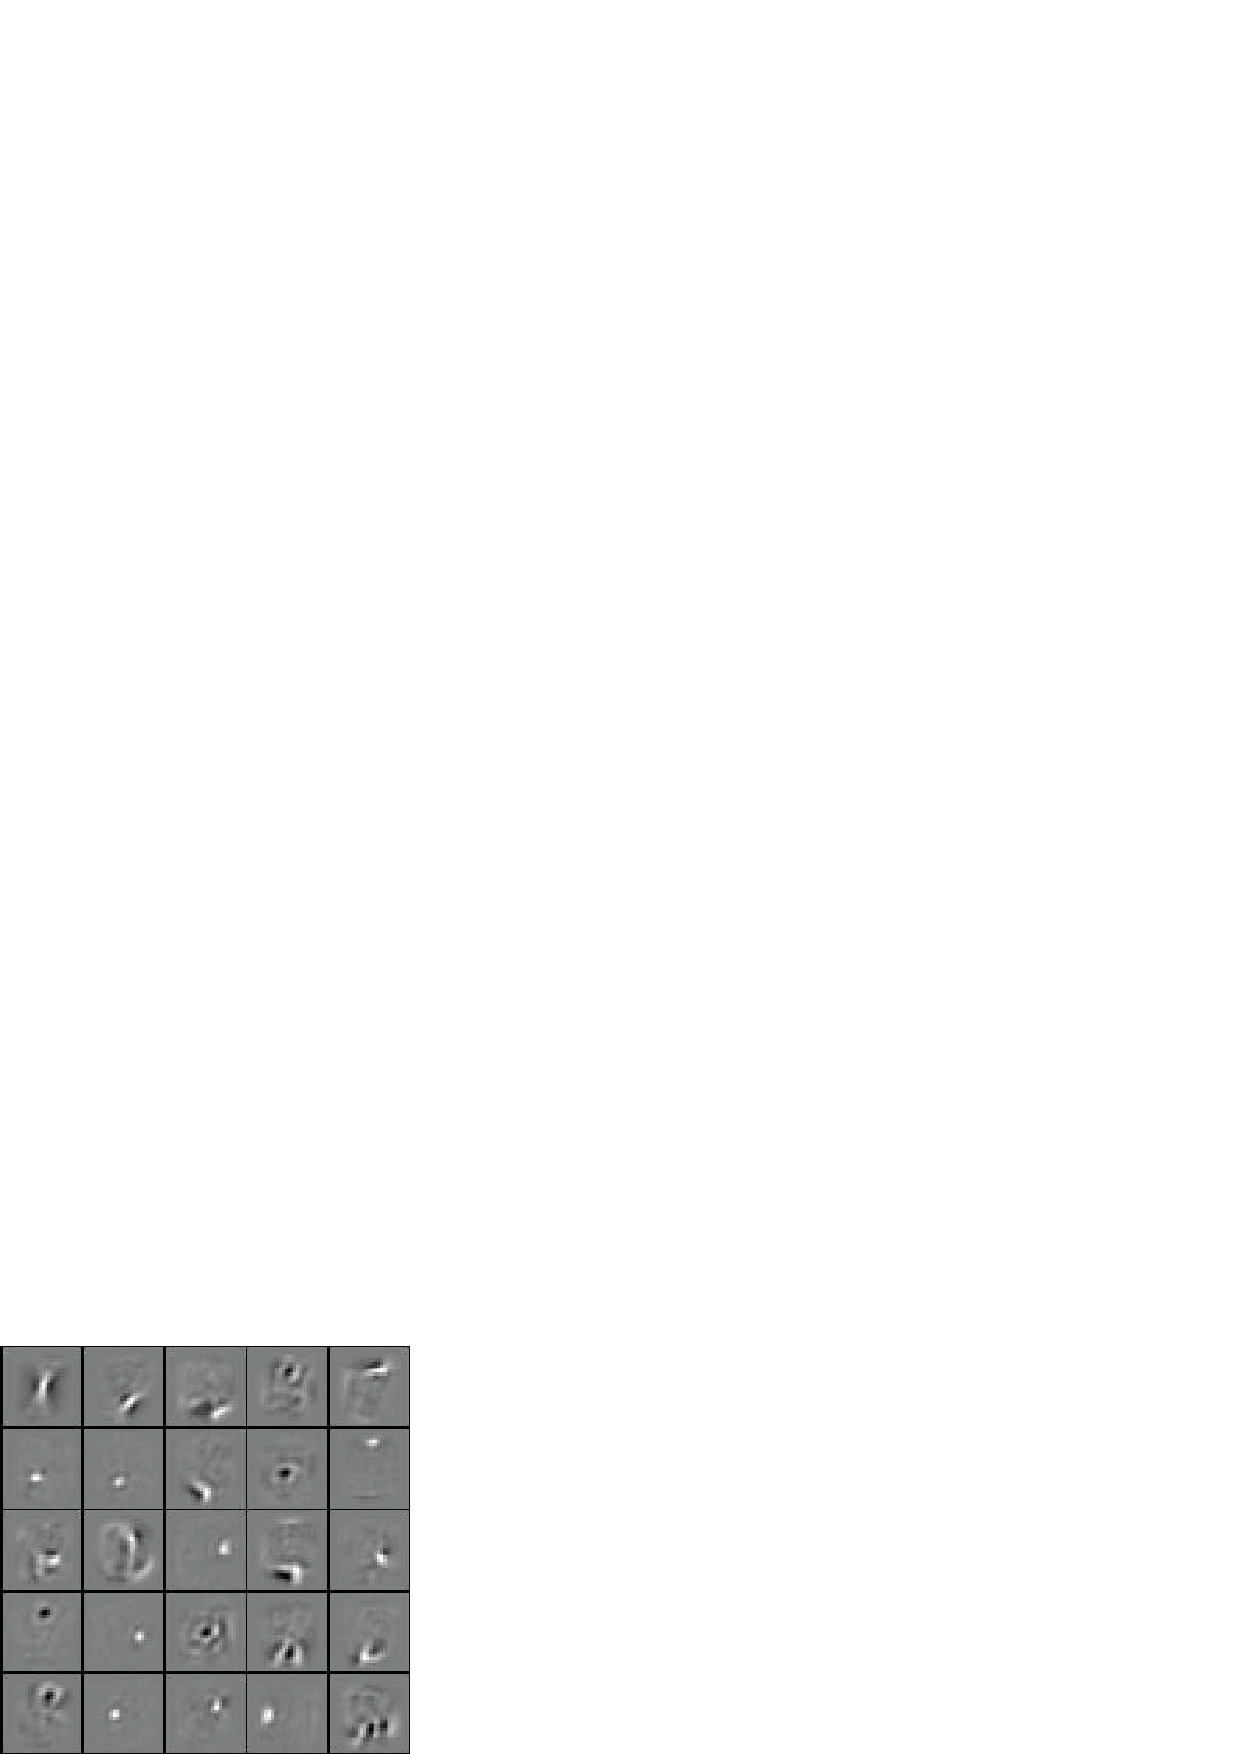
\includegraphics[scale=0.5]{./figure/weight_L1.png}
\end{minipage}
\hfill
\begin{minipage}[h]{0.8\linewidth}
\centering
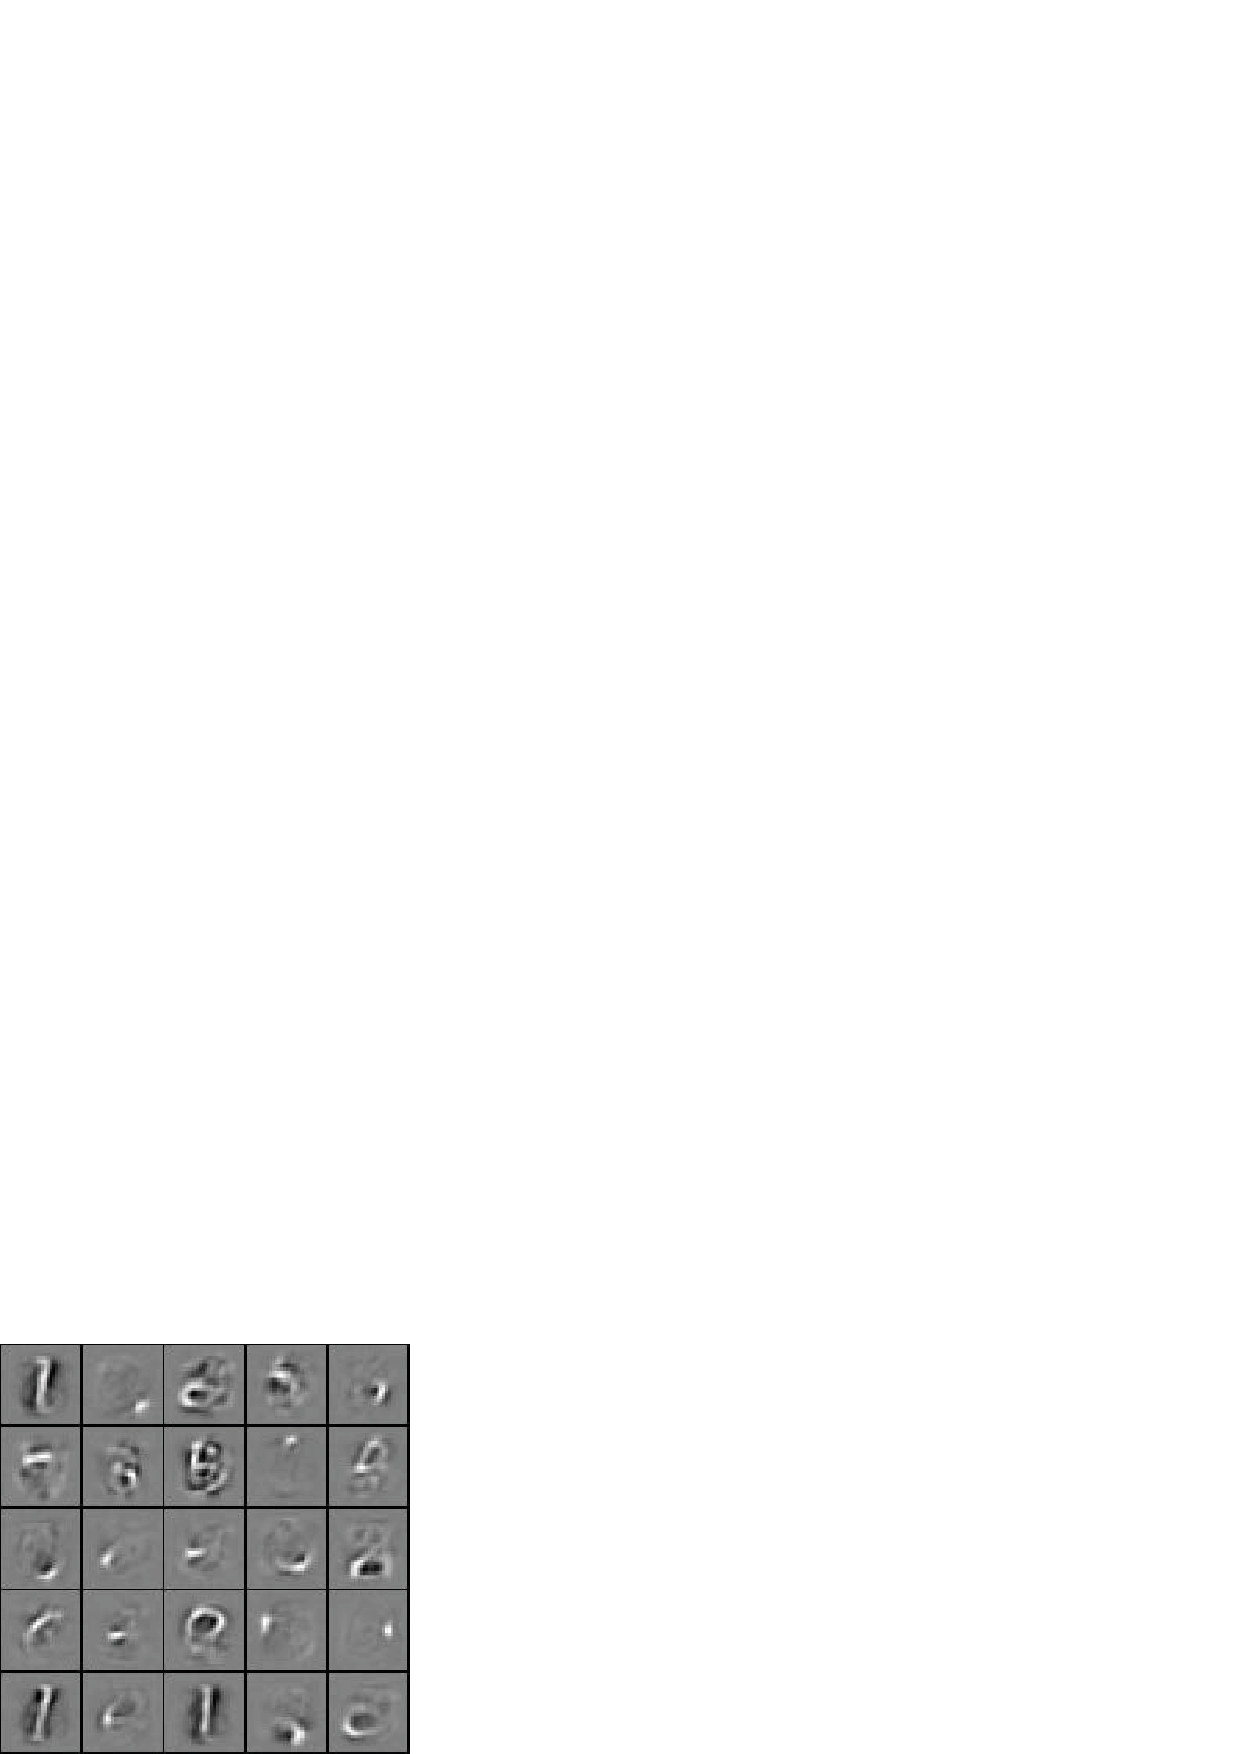
\includegraphics[scale=0.5]{./figure/weight_L2.png}
\end{minipage}
\hfill
\begin{minipage}[h]{0.8\linewidth}
\centering
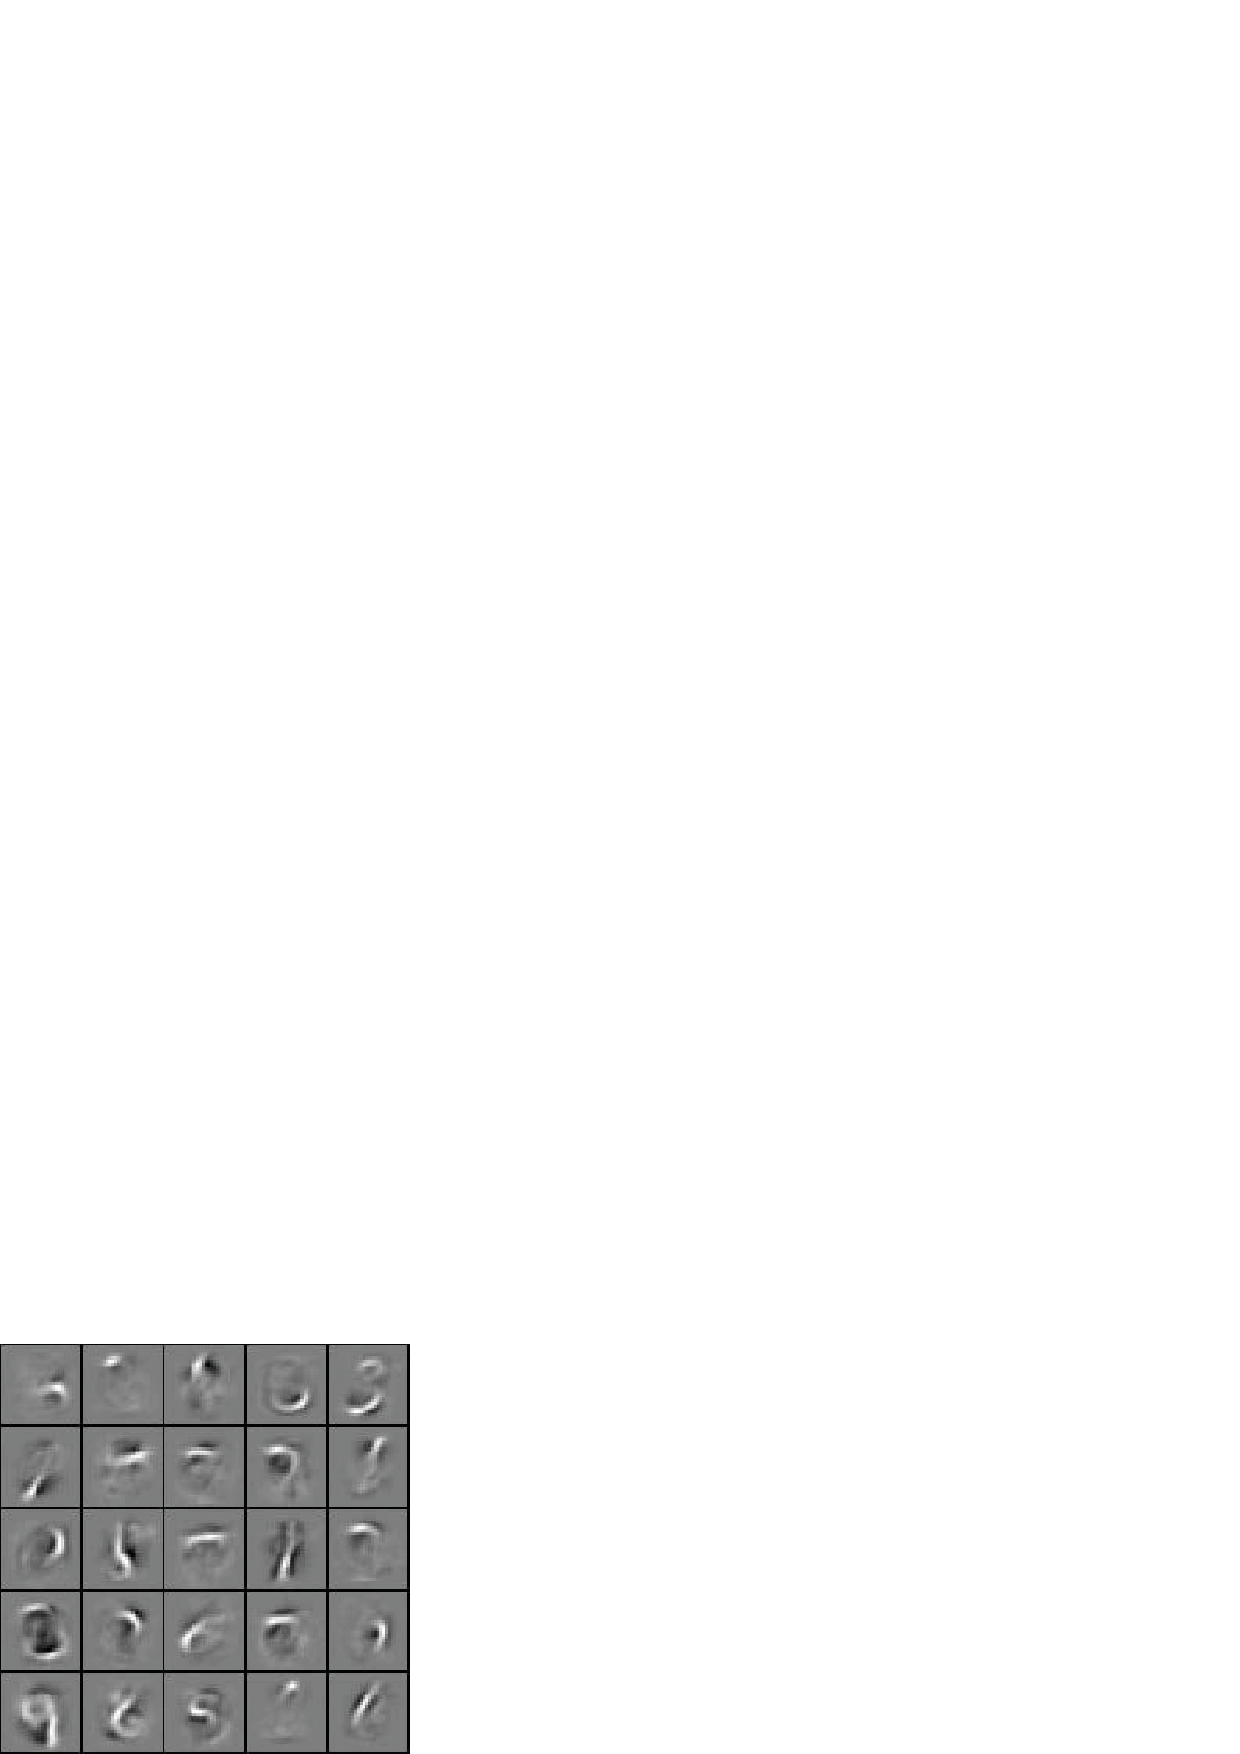
\includegraphics[scale=0.5]{./figure/weight_KL.png}
\end{minipage}
\hfill
\begin{minipage}[h]{0.8\linewidth}
\centering
\includegraphics[scale=0.5]{./figure/MNIST_student_weight.eps}
\end{minipage}
\end{figure}


在图 \ref{fig:st}和\ref{fig:kl} 中,由KL因子和Student-t 因子自动编码器能训练获得一些浅层的局部特征。若将这些特征用于深层神经网络(DNN)能较好地完成工作。与此同时,L2范数因子自动编码器能训练获得一些全局的特征,能直接用于简单的浅层分类器,达到有效的精确率,如图\ref{fig:l2}所示。然而,L1 范数自动编码器生成的特征效果明显差于其它的惩罚因子,特征模糊不明显。最后,所有稀疏编码器获得的特征均比纯自动编码器的好,纯自动编码器的特征看上去杂乱无章,表明使用稀疏惩罚因子能有效提高特征的区分度。



\section{实验数据分析}
实验数据整理,如下图\label{fig:sparsitylevel} 所示,每行四张图对应一个数据集上的实验,按照行顺序为:MNIST、CIFAR-10、SVHL-10、OPTDIGITS、NORB数据集。对于一个数据集,我们采用四个不同的稀疏惩罚因子分别进行实验,按照从左到右的顺序为:L1范数、L2范数、KL因子、Student-t因子。其中左边栏表示特征的稀疏度,右边栏表示测试集上的正确率,X轴表示稀疏参数的取值范围。
\begin{figure}[h]	  
\caption{不同稀疏惩罚因子的模型的稀疏度、正确率统计图表\label{fig:sparsitylevel}}
\begin{minipage}[h]{0.23\linewidth}
\centering
\includegraphics[width=1\textwidth]{./figure/MNIST_L1.eps}
\end{minipage}
\hfill
\begin{minipage}[h]{0.24\linewidth}
\centering
\includegraphics[width=1\textwidth]{./figure/MNIST_L2.eps}
\end{minipage}
\hfill
\begin{minipage}[h]{0.24\linewidth}
\centering
\includegraphics[width=1\textwidth]{./figure/MNIST_student.eps}
\end{minipage}
\hfill
\begin{minipage}[h]{0.24\linewidth}
\centering
\includegraphics[width=1\textwidth]{./figure/MNIST_KL.eps}
\end{minipage}
\hfill
\begin{minipage}[h]{0.24\linewidth}
\centering
\includegraphics[width=1\textwidth]{./figure/cifar_L1.eps}
\end{minipage}
\hfill
\begin{minipage}[h]{0.24\linewidth}
\centering
\includegraphics[width=1\textwidth]{./figure/cifar_L2.eps}
\end{minipage}
\hfill
\begin{minipage}[h]{0.24\linewidth}
\centering
\includegraphics[width=1\textwidth]{./figure/cifar_student.eps}
\end{minipage}
\hfill
\begin{minipage}[h]{0.23\linewidth}
\centering
\includegraphics[width=1\textwidth]{./figure/cifar_KL.eps}
\end{minipage}
\hfill
\begin{minipage}[h]{0.24\linewidth}
\centering
\includegraphics[width=1\textwidth]{./figure/svhn_L1.eps}
\end{minipage}
\hfill
\begin{minipage}[h]{0.24\linewidth}
\centering
\includegraphics[width=1\textwidth]{./figure/svhn_L2.eps}
\end{minipage}
\hfill
\begin{minipage}[h]{0.24\linewidth}
\centering
\includegraphics[width=1\textwidth]{./figure/svhn_student.eps}
\end{minipage}
\hfill
\begin{minipage}[h]{0.24\linewidth}
\centering
\includegraphics[width=1\textwidth]{./figure/svhn_KL.eps}
\end{minipage}
\hfill
\begin{minipage}[h]{0.24\linewidth}
\centering
\includegraphics[width=1\textwidth]{./figure/optdigits_L1.eps}
\end{minipage}
\hfill
\begin{minipage}[h]{0.24\linewidth}
\centering
\includegraphics[width=1\textwidth]{./figure/optdigits_L2.eps}
\end{minipage}
\hfill
\begin{minipage}[h]{0.24\linewidth}
\centering
\includegraphics[width=1\textwidth]{./figure/optdigits_student.eps}
\end{minipage}
\hfill
\begin{minipage}[h]{0.24\linewidth}
\centering
\includegraphics[width=1\textwidth]{./figure/optdigits_KL.eps}
\end{minipage}
\hfill
\begin{minipage}[h]{0.24\linewidth}
\centering
\includegraphics[width=1\textwidth]{./figure/norb_L1.eps}
\end{minipage}
\hfill
\begin{minipage}[h]{0.24\linewidth}
\centering
\includegraphics[width=1\textwidth]{./figure/norb_L2.eps}
\end{minipage}
\hfill
\begin{minipage}[h]{0.24\linewidth}
\centering
\includegraphics[width=1\textwidth]{./figure/norb_student.eps}
\end{minipage}	
\hfill
\begin{minipage}[h]{0.24\linewidth}
\centering
\includegraphics[width=1\textwidth]{./figure/norb_KL.eps}
\end{minipage}		
\end{figure}

从上面的图表数据我们分析得知,稀疏表示能有效提高分类精度,但在某些情况下该结论并不成立。若是特征过于稀疏,那将会压制系统的准确率。对于L1范数惩罚因子,它的稀疏度快速收敛至1,从而特征向量将会过于稀疏,导致模型的精度急剧下降。即,L1范数对系统模型的约束越小,系统的性能表现越好。另外,KL差分因子的稀疏度在每个数据集上均能平稳收敛至0.5。它的准确率和稀疏度在测试数据集上的表现均远远优于其它惩罚因子,处在一个能广泛接受的范围内。


针对系数敏感度, Student-t惩罚因子和L2 范数惩罚因子对其参数十分敏感,然而KL惩罚因子并不是这样。若我们合理调节Student-t惩罚因子和L2范数惩罚因子的系数,二者也能实现媲美KL惩罚因子的正确率。令人失望的是,L1范数对参数十分敏感,而且其在分类误差方面远远落后于其它惩罚因子,尽管它能实现更加稀疏的特征向量。

表格\ref{tab:result_mnist}, \ref{result_svhn}, \ref{result_cifar}, \ref{result_norb}和 \ref{result_optdigits} 统计了每一个稀疏惩罚因子在MNIST, CIFAR-10, SVHN, OPTDIGITS, 和 NORB 数据集上的最佳的稀疏度,正确率和重构误差。

首先,在所有包含稀疏惩罚因子的模型中,测试数据集上的重构误差都非常小,表明了autoencoder模型结构可以降低泛化误差。出人意料的是,没有任何稀疏惩罚因子的纯autoencoder在这个评价指标在大多数数据集上,获得的最好成绩。但是,它在其它评价指标上远远落后于其它模型,表明稀疏惩罚因子对整个模型的贡献。

其次,KL惩罚因子表现远远比其它简单的形式稀疏惩罚因子的测试精度和稀疏方面更好。也就是说,KL惩罚因子描述数据的概率分布模型方面比其它因子更好。此外,Student-t惩罚因子的表现是高于平均水平。考虑到其具有较强的鲁棒性,如图\ref{fig:sparsitylevel}已经表明,相较L1范数和L2范数,在产生有用稀疏特征矢量方面更可靠高效。

第三,由于原始数据集和权重矩阵的随机初始化,引入外部噪声进入模型结构,影响到评价指标的凸优化程序和性能。其结果是,在图\ref{fig:sparsitylevel},绘制的图线不光滑,在实验上OPTDIGITS更加明显,因为我们做很多的试验。总之,越重的稀疏惩罚因子的权重越大,在其评价度量幅度振荡越严重。
\begin{table}[h]
\begin{center}
{
\caption{MNIST数据集上分类精度统计表格}\label{tab:result_mnist}}
\begin{tabular}{|c|c|c|c|}
\hline
稀疏因子 & 准确率 & 稀疏度 & 重构误差 \\
\hline
Autoencoder    & 93.11\% & 0.163100   & 0.012760 \\
\hline
With L1 norm   & 95.24\% & 0.463012 & \textbf{0.006770} \\
\hline
With L2 norm   & 96.71\% & 0.484919 & 0.007998 \\
\hline
With Student-t & 96.64\% & 0.515713 & 0.008376 \\
\hline
With KL        & \textbf{97.26\%} & \textbf{0.591793} & 0.009167 \\
\hline
\end{tabular}
\end{center}
\end{table}

\begin{table}[h]
\begin{center}
{
\caption{CIFAR-10数据集上分类精度统计表格}\label{result_cifar}}
\begin{tabular}{|c|c|c|c|}
\hline
稀疏因子 & 准确率 & 稀疏度 & 重构误差 \\
\hline
Autoencoder    & 43.21\%   & 0.136970 & \textbf{0.004841} \\
\hline
With L1 norm   & 44.58\%   & 0.171718 & 0.004927 \\
\hline
With L2 norm   & 45.37\%   & 0.384946 & 0.005447 \\
\hline
With Student-t &  44.86\%  & 0.333247 & 0.005194 \\
\hline
With KL  & \textbf{48.50\%} & \textbf{0.487786} & 0.008363 \\
\hline
\end{tabular}
\end{center}
\end{table}

\begin{table}[h]
\begin{center}
{
\caption{SVHN数据集上分类精度统计表格}\label{result_svhn}}
\begin{tabular}{|c|c|c|c|}
\hline
稀疏因子 & 准确率 & 稀疏度 & 重构误差 \\
\hline
Autoencoder    & 33.45\% & 0.352854 & \textbf{0.002179} \\
\hline
With L1 norm   & 39.08\% & \textbf{0.597836} & 0.002648 \\
\hline
With L2 norm   & 51.51\% & 0.548746 & 0.003746 \\
\hline
With Student-t & 51.28\% & 0.581199 & 0.002762 \\
\hline
With KL        & \textbf{66.30\%} & 0.386963 & 0.002229\\
\hline
\end{tabular}
\end{center}
\end{table}

\begin{table}[h]
\begin{center}
{
\caption{OPTDIGITS数据集上分类精度统计表格 }\label{result_optdigits}}
\begin{tabular}{|c|c|c|c|}
\hline
稀疏因子 & 准确率 & 稀疏度 & 重构误差 \\
\hline
Autoencoder    & 93.60\%  & 0.168249 & 0.012551 \\
\hline
With L1 norm   & 93.77\%  & 0.170865 & \textbf{0.012528} \\
\hline
With L2 norm   & 93.38\%  & 0.294789 & 0.013431\\
\hline
With Student-t & 93.77\%  & 0.271513 & 0.013083 \\
\hline
With KL        & \textbf{94.49}\%  & \textbf{0.327701} & 0.013331 \\
\hline
\end{tabular}
\end{center}
\end{table}

\begin{table}[h]
\begin{center}
{
\caption{NORB数据集上分类精度统计表格}\label{result_norb}}
\begin{tabular}{|c|c|c|c|}
\hline
稀疏因子 & 准确率 & 稀疏度 & 重构误差 \\
\hline
Autoencoder    & 72.88\%  & 0.234830 & 0.001241 \\
\hline
With L1 norm   & 75.65\%  & \textbf{0.552909} & 0.001268 \\
\hline
With L2 norm   & 76.92\%  & 0.543356 & 0.001260 \\
\hline
With Student-t & 75.72\% & 0.548898 & 0.001256 \\
\hline
With KL        & \textbf{83.05}\%  & 0.269471 & \textbf{0.001140} \\
\hline
\end{tabular}
\end{center}
\end{table}



\chapter{总结}
\section{完成的工作}
非监督学习手段能适应现实世界复杂的处理需求,传统的人工手段和机器学习方法需要手动设计特征提取手段,然而这些设计技巧不具有通用性,无法针对复杂的图像、视频、音频进行有效的处理。本文对非监督学习方法中的稀疏自动编码器模型进行了研究,并对探讨了稀疏惩罚因子对模型的精确度、特征提取的有效性的影响。本文的主要研究工作如下:

(1)对近年来深度学习的发展做了总结,并对该领域的相关科技文献做了归纳。深度学习起源于人工神经网络,通过组合低层特征形成更加抽象的高层表示(属性类别或特征),以发现数据的分布式特征表示。它能有效应对``维数灾难''和``局部泛化限制''等问题,传统的机器学习方法容易出现过拟合现象,导致模型不能适应更加复杂的情形。近年来,该领域的工作哦取得了较大的进展,该领域中主要的深度结构:深度信念网络(DBN),限制玻尔兹曼机(RBM),稀疏自动编码器(SAE)在语音处理、图像识别和视频分析中取得了开拓性研究进展。研究这些文献资料对理解稀疏自动编码器的模型架构具有重大借鉴意义。

(2)实现了Andrew Ng 提出的自学习算法(Self-Taught Learning),即利用稀疏自动编码器实现特征提取,在利用Softmax分类器对特征进行训练,获得一个更加高效的分类器。其中,提取由自动编码器到的特征的质量对后续的分类器的精度影响巨大,故引用文献中的计算公式来评价``稀疏特征''有效性。另一方面,我们采用不同的稀疏惩罚因子,例如:L1范数,KL因子,进行对照实验,期望分析出最有效的稀疏因子,以提高实验精度。

(3)利用Django技术搭建实验提交平台,以便用户提交实验计算任务,查看任务进度和分析实验结果。同时开放实验预处理环节,以供用户自行抉择。后台采用 MATLAB 计算框架实现,完成用户提交的实验计算需求,并将实验结果利用 Chat.js 插件绘制图像表格,同时也提供 MATLAB 的EPS图像绘制方法。由于 MATLAB 自带的图表绘制系统更为专业,同时可以定制代码,显示特定格式的图表。所以相对于采用 WEB 框架中的JS插件,利用实验数据结果绘制美观的图表,采用 MARLAB 的plot函数更能满足科研需求。


\section{存在的问题及下一步工作}
经过四年的本科学习,我初步掌握了计算机的专业知识和基本技能,在最后一学期的实践环节中,经过几个月的设计与实现,基本完成了前台的WEB界面框架和后台的MATLAB算法框架。其功能基本符合用户需求,能后完成用户在线提交计算任务,自动完成任务计算,并展示任务结果等功能。由于毕业设计时间较短,网站框架掌握不全,所以该应用还有许多不尽如人意的地方,如:。今后的网站应用将进一步优化完善前台界面和后台对应功能支持,以保证能解构更多的计算任务需求,以更好地为用户提供计算服务。

\backmatter
%%%%%%%%%%%%%%%%%%%%%%%%%%%%%%
%% 参考文献
%%%%%%%%%%%%%%%%%%%%%%%%%%%%%%
\ZJUthesisbib{thesisbib}

\begin{thanks}
~~~~~~~~毕业设计得以顺利完成,除了我自己一年来的潜心学习和研究之外,也凝聚了很多人的心血。所以在这里,我要对帮助我顺利完成毕业设计的所有人表示感谢。我要对我指导老师——浙江工业大学龙胜春老师以及北京航空航天大学荣文戈老师,表示我最由衷的感谢。本课题在选题及开发过程中得到龙老师和荣老师的悉心指导。龙老师把关督促毕业设计的进展,并为指点,帮助我开拓研究思路,热忱鼓励。龙老师一丝不苟的作风,严谨求实的态度,踏踏实实的精神一直是我的榜样。另外还要感谢我的同伴和在实践中帮助过我的同学,使我能顺利完成毕业设计。感谢其他同学和老师,感谢浙江工业大学,在毕业设计开发过程中提供良好工作环境和气氛。
\end{thanks}


\appendix
\chapter{附录}
\textbf{附录1~ 毕业设计文献综述}

\textbf{附录2~ 毕业设计开题报告}

\textbf{附录3~ 毕业设计外文翻译(中文译文与外文原文)}


\ZJUindex


\end{document}

